\chapter{Neutrino Interactions}
\label{ch:neutrino_interactions}


While the previous chapter described neutrino oscillations and the challenges for current and future neutrino oscillation experiments due to neutrino-nucleus interactions, this chapter focuses on neutrino interactions, describing the approximations used and the models employed in neutrino simulations. The different neutrino interaction modes are described in Section \ref{sec:interaction_modes}, and the nuclear effects due to the neutrino-nucleus interaction are shown in Section \ref{sec:nuclear_effects}. Finally, Section \ref{sec:remarks} shows a summary and the need for more measurements, introducing the $\nu_\mu$ \acrshort{cc} measurement on argon that will be described in this thesis.



\section{Neutrino Interaction Modes}
\label{sec:interaction_modes}


\begin{figure}[t]
\centering
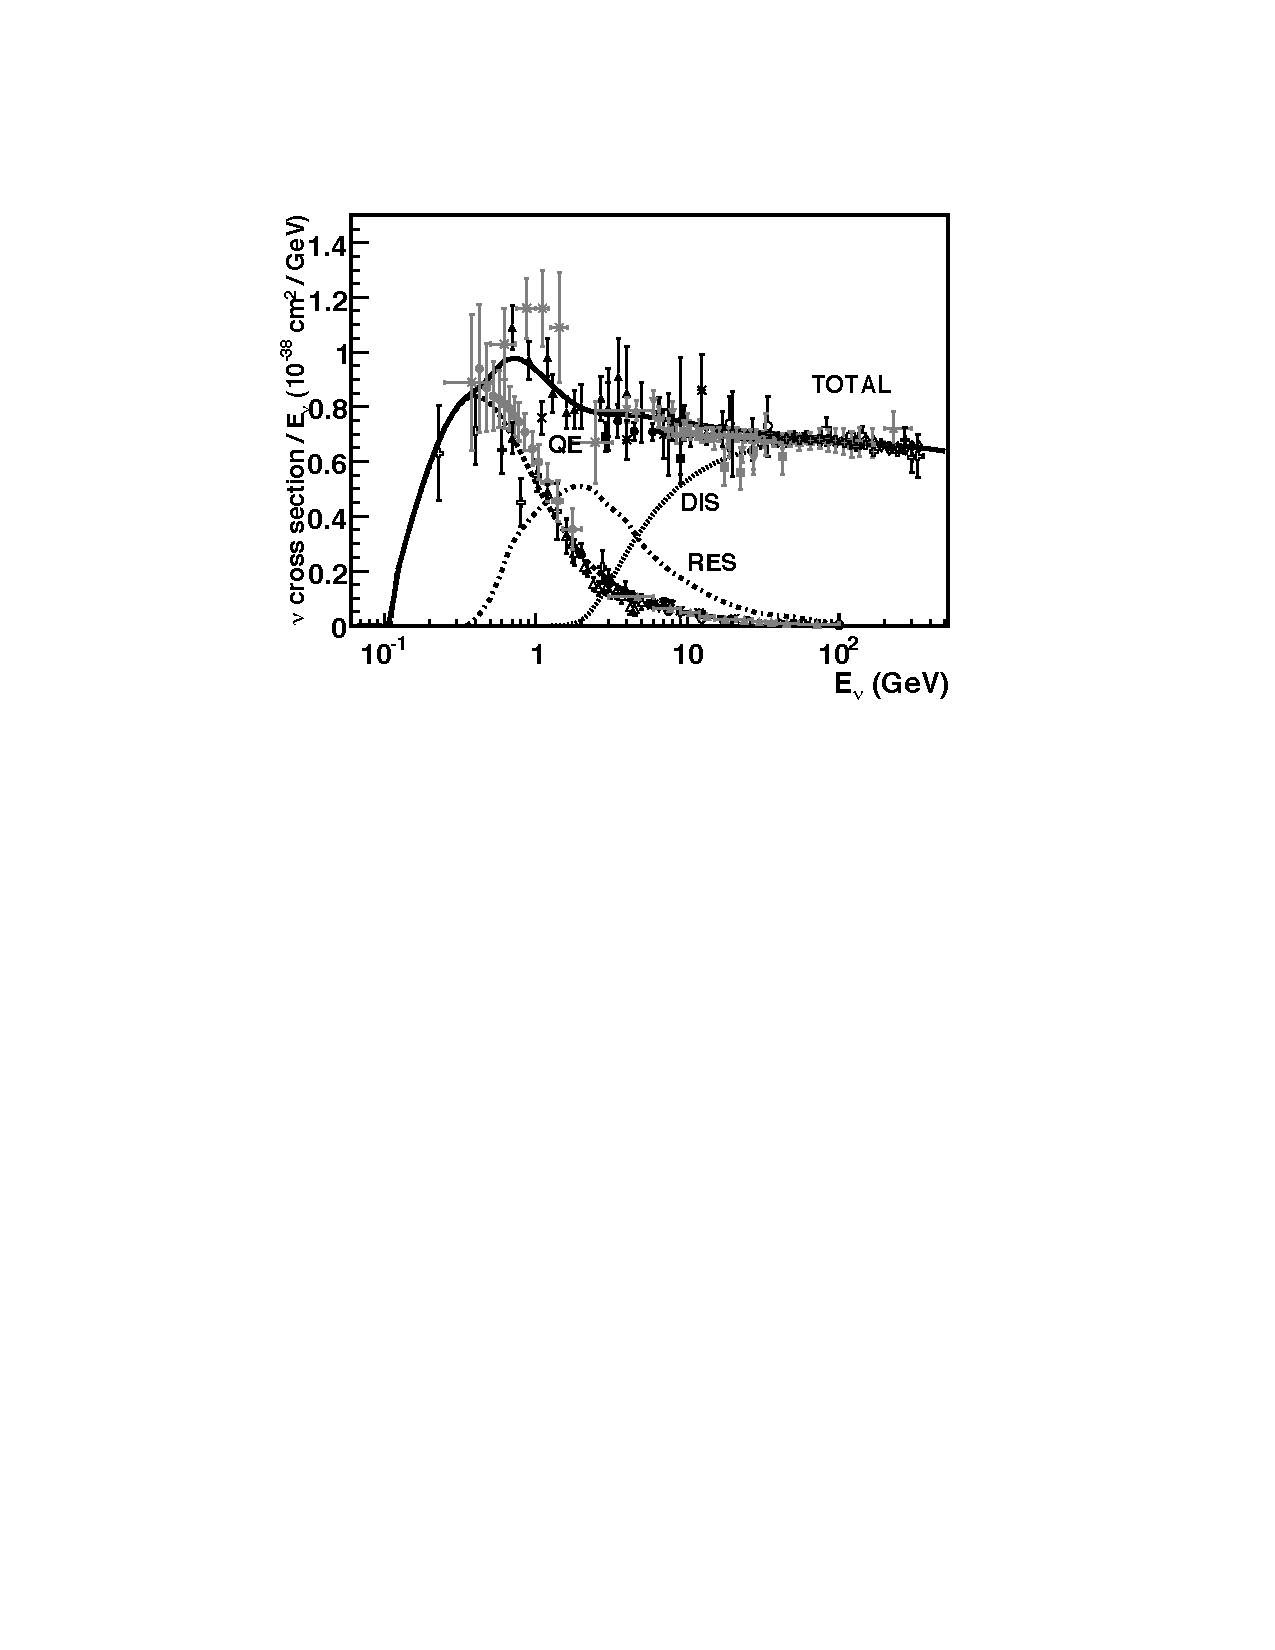
\includegraphics[width=.70\textwidth]{images/NeutrinoInteractions/all_xsec}
\caption[$\nu_\mu$ Charged Current Cross Section Measurements]{Total neutrino per nucleon \acrshort{cc} cross sections (for an isoscalar target) divided by neutrino energy and plotted as a function of energy. The data points show the results of different experiments, as described in~\cite{zeller}. Also shown are the various contributing processes that will be described in the next sections. These contributions include \acrshort{qe} scattering (dashed), resonance production (dot-dash), and \acrshort{dis} scattering (dotted). Example predictions for each are provided by the NUANCE generator~\cite{nuance}. Source:~\cite{zeller}.}
\label{fig:all_xsec}
\end{figure}

The description of neutrino scattering between $0.1 - 20$ GeV can be described by several distinct neutrino scattering mechanisms~\cite{zeller}. The possibilities fall into three main categories, also shown in Figure~\ref{fig:all_xsec}:
\begin{description}
\item[Elastic and Quasi-Elastic Scattering] Neutrinos can elastically scatter off an entire nucleon liberating a nucleon (or multiple nucleons) from the target. In the case of \acrshort{cc} neutrino scattering, this process is referred to as ``\acrshort{qe} scattering'' because neutrinos become charged leptons in the final state. For \acrshort{nc} scattering, this is traditionally referred to as ``elastic scattering'', although the ``quasi elastic'' terminology is also used for \acrshort{nc} interactions, and it refers to when the final state nuclear targets are not in their ground states.
These mechanisms are described in Section~\ref{sec:qe}. 
\item[Resonance Production] Neutrinos can excite the target nucleon to a resonance state. The resultant baryonic resonance decays to a variety of possible mesonic final states producing combinations of nucleons and mesons. This is described in Section~\ref{sec:res}.
\item[Deep Inelastic Scattering] Given enough energy, the neutrino can resolve the individual quark constituents of the nucleon. This is called \acrfull{dis} and manifests in the creation of a hadronic shower. This is described in Section~\ref{sec:dis}.
\end{description}
Examples of these types of interaction are shown in Figure~\ref{fig:evd_interactions}, as they appear in a \acrshort{lartpc} detector.
As a results of all these processes, the products of neutrino interactions include a variety of final states ranging from the emission of nucleons to more complex final states including pions, kaons, and collections of mesons.
Other interaction processes, like coherent pion production and kaon production, are also present, and they will be briefly discussed in Section~\ref{sec:other_interactions}.

Looking at Figure~\ref{fig:all_xsec}, and considering that neutrinos at the MicroBooNE detector have energy from a few tens of MeV to $\sim 2$ GeV, the relevant interaction processes for the measurement in this thesis are \acrshort{qe} scattering and resonance production, with a small contribution from \acrshort{dis} events.

\begin{figure}[]
\centering
\subfloat[][$\nu_\mu$ \acrshort{cc} \acrshort{qe} candidate event.]
   {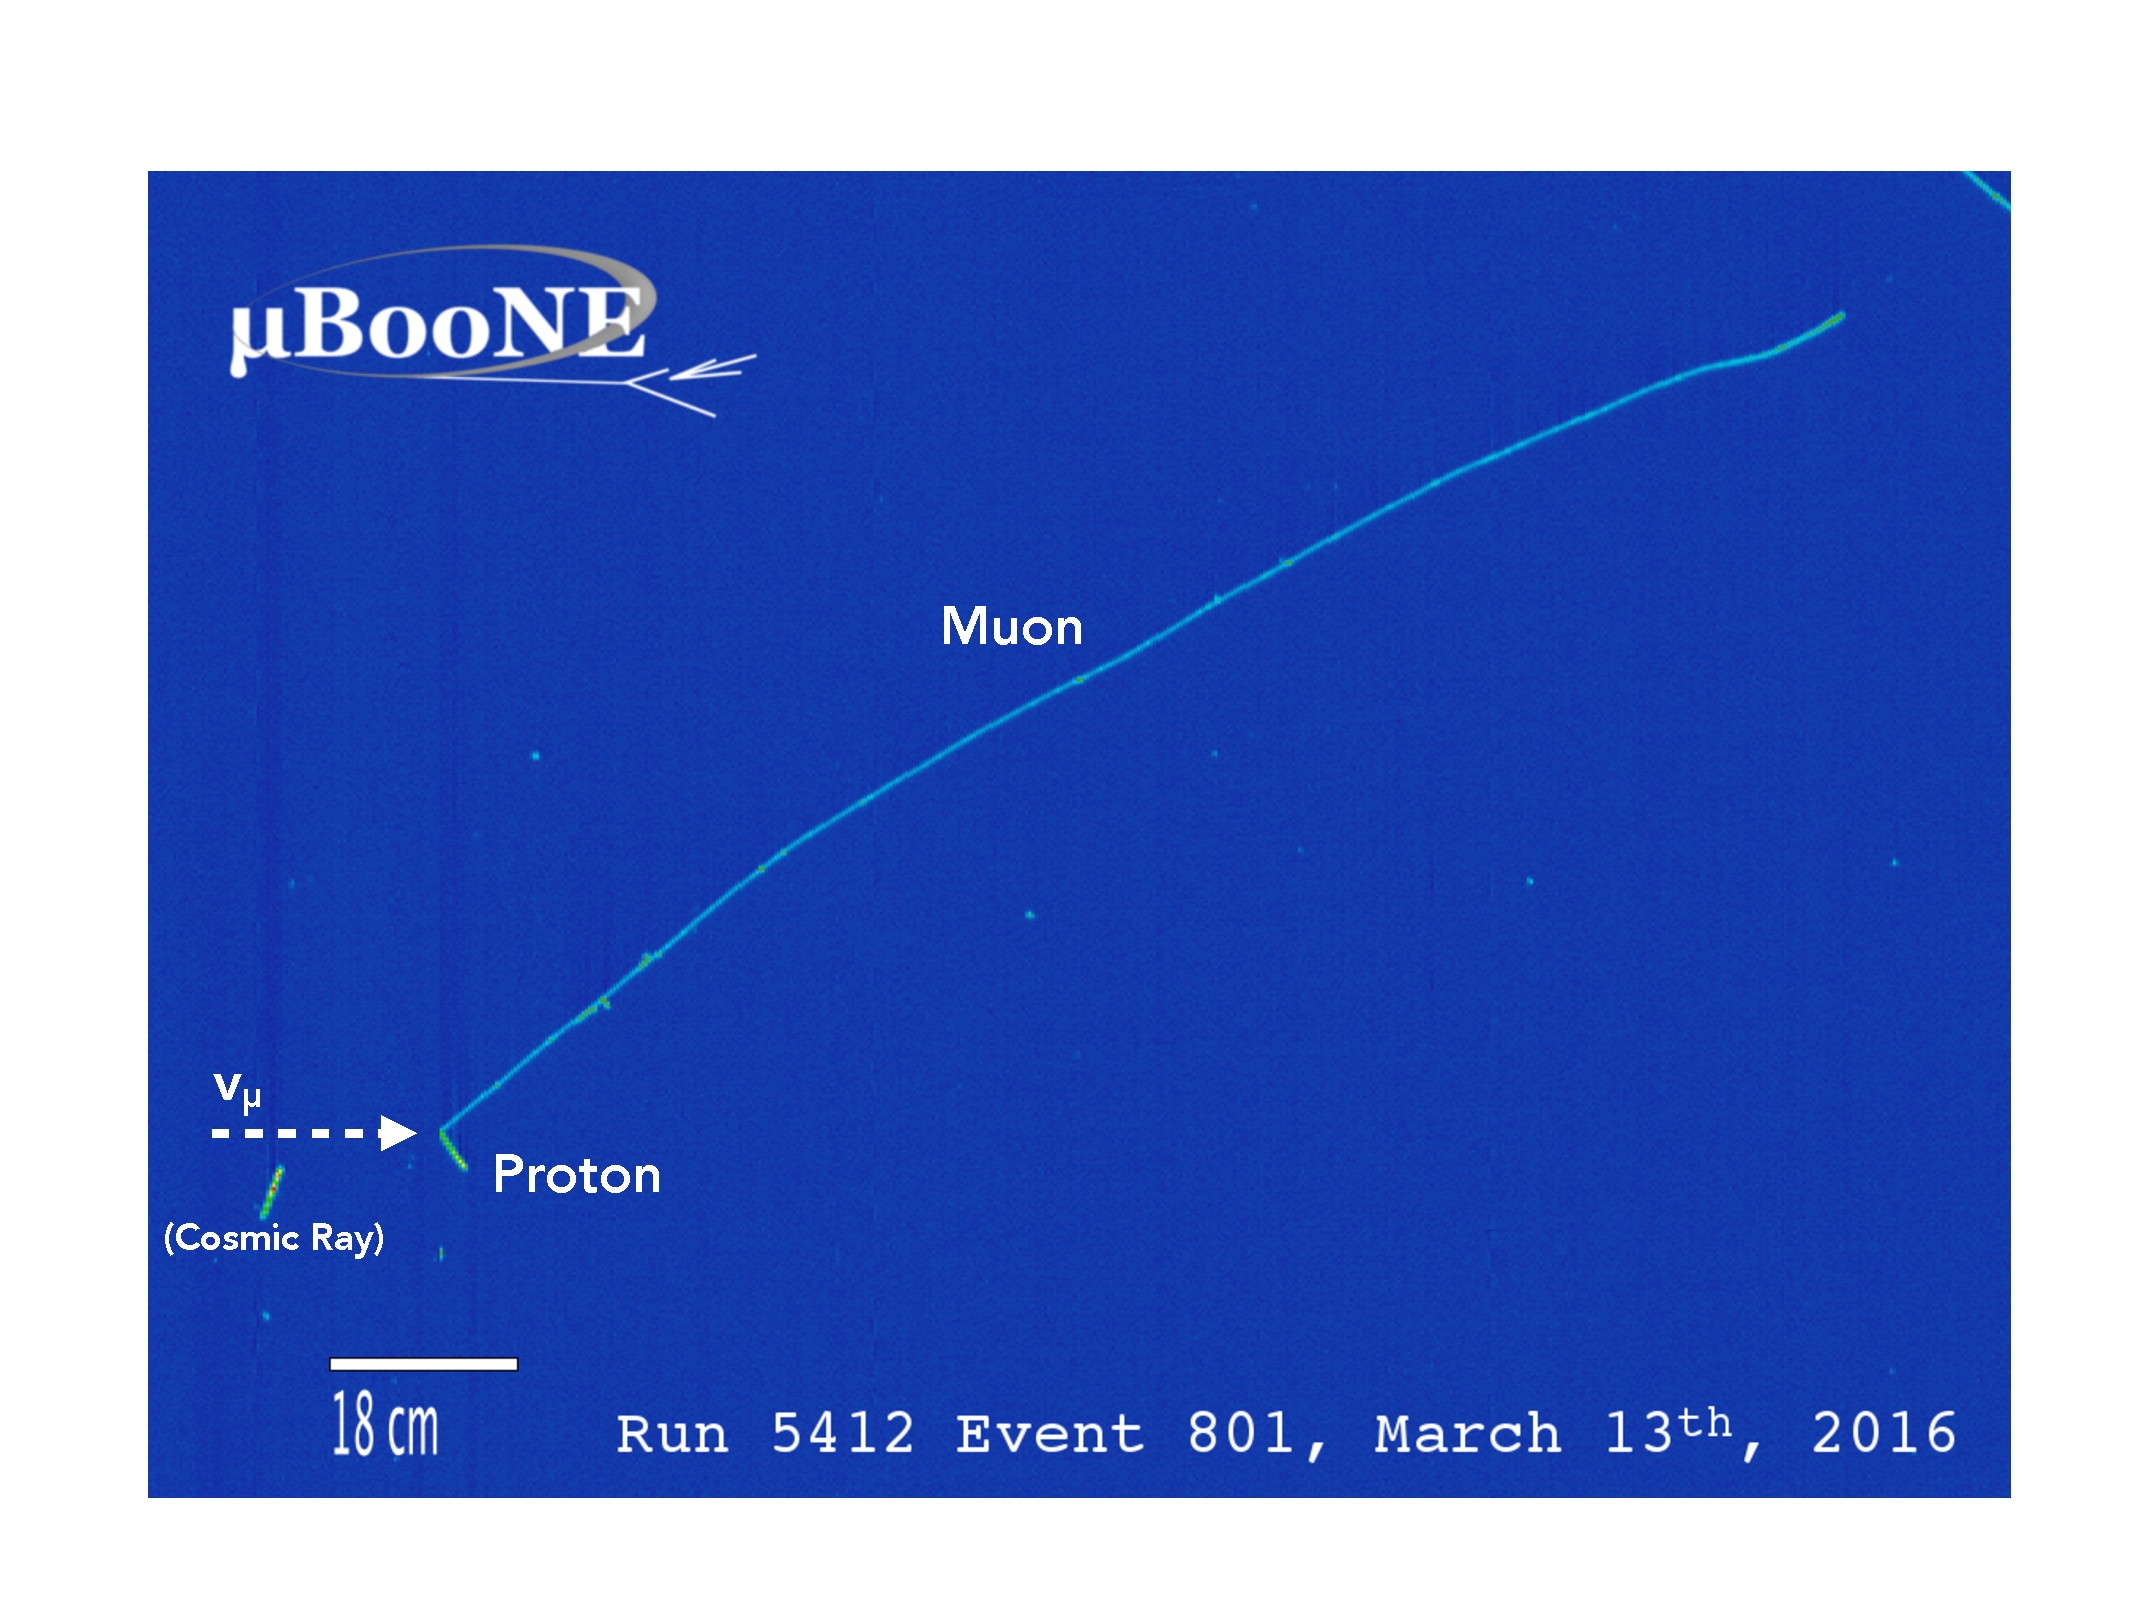
\includegraphics[width=.59\textwidth]{images/NeutrinoInteractions/evd_qe}
   \label{fig:evd_qe}} \quad
\subfloat[][$\nu_\mu$ \acrshort{cc} resonance candidate event.]
   {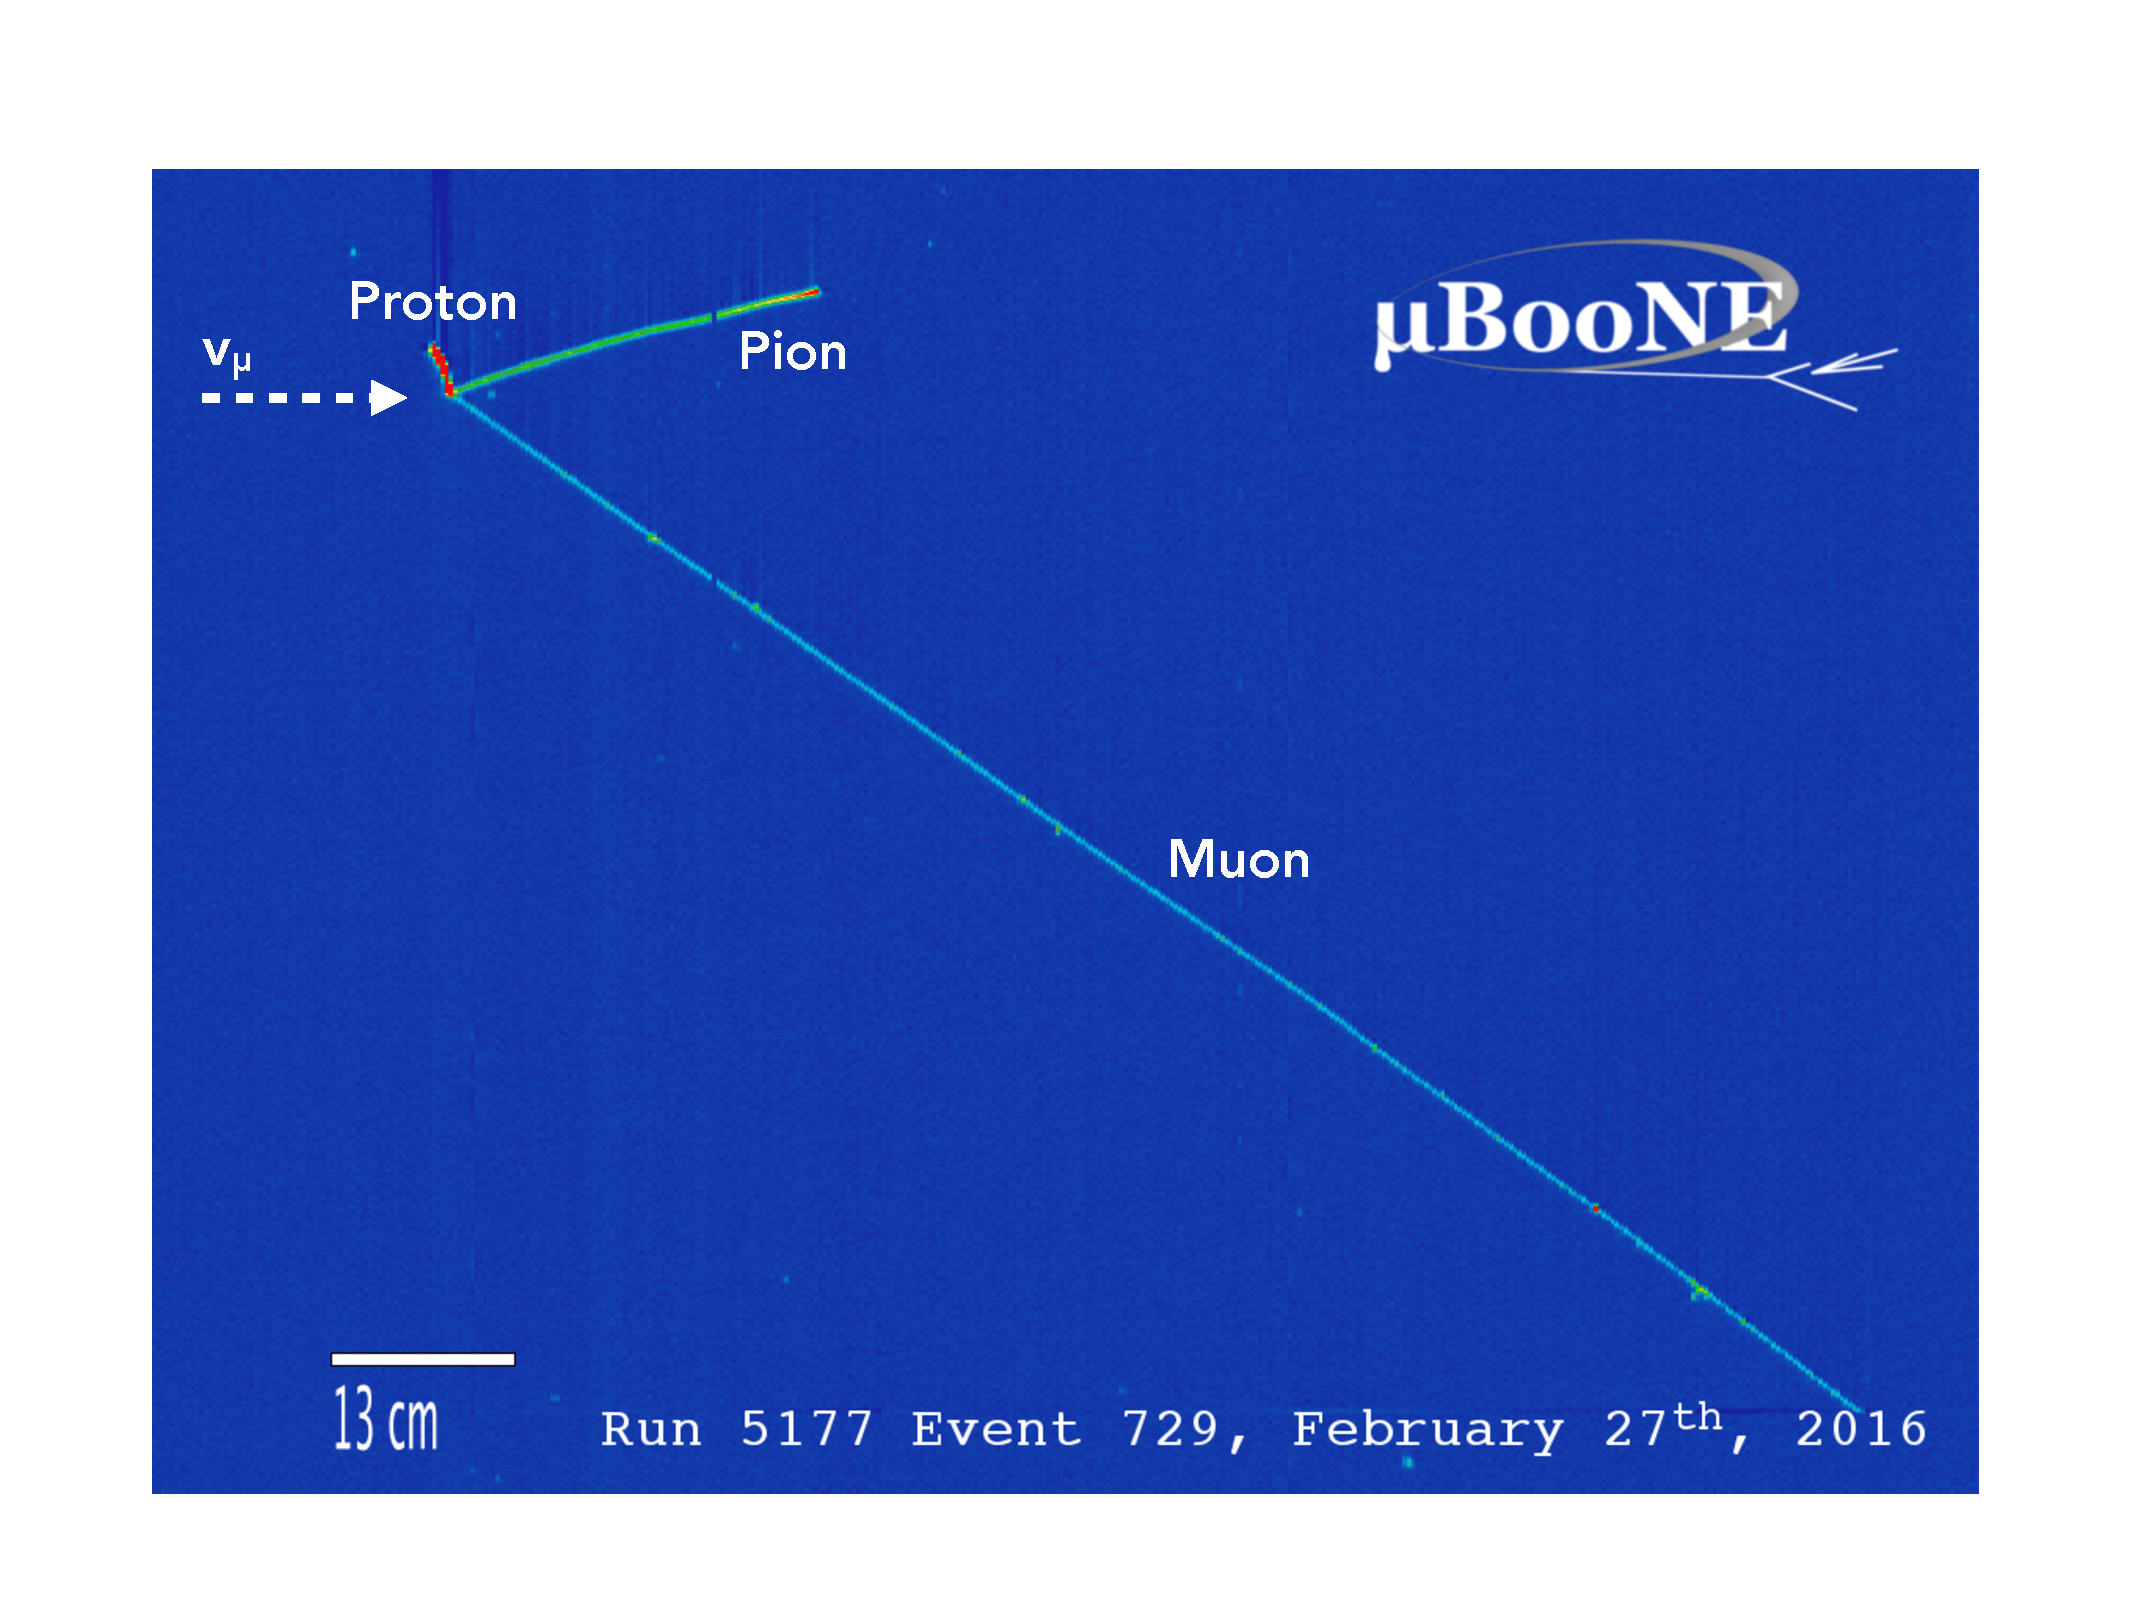
\includegraphics[width=.59\textwidth]{images/NeutrinoInteractions/evd_res}
   \label{fig:evd_res}} \quad
\subfloat[][$\nu_\mu$ \acrshort{cc} \acrshort{dis} candidate event.]
   {\includegraphics[width=.59\textwidth]{images/NeutrinoInteractions/evd_dis}
   \label{fig:evd_dis}} \\
\caption[Neutrino Interaction Modes from MicroBooNE Event Displays]{Events recorded by the MicroBooNE detector showing \acrshort{qe}~\subref{fig:evd_qe}, resonance~\subref{fig:evd_res}, and \acrshort{dis}~\subref{fig:evd_dis} events. The images show a 2D projection of the events, and display the final state particles coming from the neutrino interactions. Neutrinos come from the left. More details on the MicroBooNE event display are given in Section~\ref{sec:signal_formation}.}
\label{fig:evd_interactions}
\end{figure}





\subsection{Quasi-Elastic Interactions}
\label{sec:qe}

%+++++++++FIGURE+++++++++
% mpost fyW
% mpost fyZ
\begin{figure}[h]
\centering
\subfloat[][]
   {
   \centering
\begin{fmffile}{fyW}
  \begin{fmfgraph*}(50,50)
\fmfleft{i1,t1,t2,t3,t4,t5,t6,t7,t8,i2}
\fmfright{o1,p1,p2,p3,p4,p5,p6,p7,p8,o2} 
\fmf{fermion}{i1,vp}
\fmf{fermion}{vp,o1}
\fmf{photon,label=$W$,label.side=right}{vp,vl}
\fmf{fermion}{i2,vl}
\fmf{fermion}{vl,o2}
\fmflabel{$\nu_l$}{i2} 
\fmflabel{$l^-$}{o2}
\fmflabel{$n$}{i1} 
\fmflabel{$p$}{o1}
  \end{fmfgraph*}
\end{fmffile}
   \label{fig:diagramW}  
   } \qquad\qquad \qquad
   \subfloat[][]
   {
   \centering
 \begin{fmffile}{fyZ}
  \begin{fmfgraph*}(50,50)
\fmfleft{i1,t1,t2,t3,t4,t5,t6,t7,t8,i2}
\fmfright{o1,p1,p2,p3,p4,p5,p6,p7,p8,o2} 
\fmf{fermion}{i1,vp}
\fmf{fermion}{vp,o1}
\fmf{photon,label=$Z$,label.side=right}{vp,vl}
\fmf{fermion}{i2,vl}
\fmf{fermion}{vl,o2}
\fmflabel{$\nu_l$}{i2} 
\fmflabel{$\nu_l$}{o2}
\fmflabel{$n$}{i1} 
\fmflabel{$n$}{o1}
  \end{fmfgraph*}
\end{fmffile}
   \label{fig:diagramZ}
   } \\
\caption[Feynman Diagrams for Quasi-Elastic Scattering]{Example of Feynman diagrams of \acrshort{qe} interactions. A \acrshort{cc} with a $W$ exchange~\protect\subref{fig:diagramW}, and a \acrshort{nc} one, with a $Z$ exchange~\protect\subref{fig:diagramZ}.}
\label{fig:diagramWZ}
\end{figure}
%++++++++++++++++++++++++

At neutrino energies between $\sim0.1$ and $\sim1.5$ GeV, the primary way in which neutrinos interact with matter is via \acrshort{qe} interactions, as shown in Figure~\ref{fig:diagramWZ}. These interactions will now be discussed in details, as MicroBooNE deals with neutrinos mainly at these energies.
This section focuses on \acrshort{cc} interactions, which include the following processes: 
\begin{equation}
\nu_l + n \rightarrow l^- + p, \qquad \bar{\nu}_l + p \rightarrow l^+ + n,
\end{equation} 
for lepton flavour $l$, a neutron $n$ and proton $p$.


%Uncertainties in the neutrino interaction model are the largest uncertainties affecting the normalisation of events in the SBN detectors,
%
%Neutrino interactions on argon are simulated using the \g neutrino event generator. \g simulates each stage of the interaction including inclusive and exclusive differential cross sections off individual nucleons and the effects of the nuclear medium on final state particles as they propagate out of the target nucleus (final state interactions).

%Multi-nucleon correlation effects of the initial state are also a challenge in neutrino interactions and are not part of the present simulation.


Starting from Equation~\eqref{eqn:lagrangian}, an effective \acrshort{cc} Lagrangian can be written by requiring that the squared momentum transferred being smaller than the $W$ mass squared, $q^2 \ll M_W^2$, and so integrating out the $W$ boson, and by working at the first order in perturbation theory \cite{halzen}: 
\begin{equation}
\mathcal{L}_\text{eff} = - \frac{G_F}{\sqrt{2}} \left ( J^{\mu} {J_\mu}^\dagger \right ),
\end{equation}
where $G_F$ is the Fermi constant. The current $J^{\mu}$ is given by
\begin{equation}
J^{\mu} = \sum_l \bar{\nu}_l\gamma^\mu(1-\gamma^5)l + \sum_{ij} V_{ij}^\text{CKM} \bar{U}_i\gamma_\mu(1-\gamma_5)D_j,
\end{equation}
where $\nu_l$ and $l$ are the neutrino and lepton spinors with flavour $l$, $V^\text{CKM}$ is the Cabibbo–Kobayashi–Maskawa (CKM) matrix for the quark mixing, and $U$ and $D$ denote the up- and down-type quark spinors respectively.

%At the energy scales of QE interactions, the neutrino is not able to resolve the partons in the nucleon, but it rather interacts with the nucleon as a whole. Given the lack of knowledge of quantum-cromodynamics (QCD)  at low energy, it is not possible to analytically evaluate the neutrino cross section with protons and neutrons.
%Cross sections are then parametrised with ``form factor'' which effectively take into account the internal structure of the nucleons as well as their coupling with the lepton current.

The above Lagrangian describes the quark-level interaction as shown in Figure~\ref{fig:fyW_a}, but in reality, it is not possible to study neutrino interactions with free quarks, but rather with neutrons or protons. While the lepton current can be calculated exactly, this is not the case for the hadronic current. Problems arise in this case given the ignorance on the internal structure of the nucleons, and the inability to solve \acrfull{qcd} at low energies. 
Cross sections are then parametrised with ``form factors'' which effectively take into account the internal structure of the nucleons as well as their coupling with the lepton current, as schematically shown in Figure~\ref{fig:fyW_b}.
%For hadrons and nucleons, effective interactions are needed to parametrise this ignorance, as schematically shown in Figure~\ref{fig:fyW_b}.

% mpost fyW_a
% mpost fyW_b
\begin{figure}[]
\centering
\subfloat[][]
   {
   \centering
\begin{fmffile}{fyW_a}
  \begin{fmfgraph*}(40,25)
    \fmfleft{i1,i2}
    \fmfright{o1,o2}
    \fmftop{b}
    \fmf{fermion}{i1,v1,o1}
    \fmf{photon}{v1,b}
    \fmflabel{$q$}{i1}
%    \fmflabel{i2}{i2}
    \fmflabel{$q'$}{o1}
%    \fmflabel{o2}{o2}
    \fmflabel{$W$}{b}
  \end{fmfgraph*}
\end{fmffile}
   \label{fig:fyW_a}  
   } \qquad \qquad $\longrightarrow$ \qquad \qquad
   \subfloat[][]
   {
   \centering
\begin{fmffile}{fyW_b}
  \begin{fmfgraph*}(40,25)
    \fmfleft{i1,i2}
    \fmfright{o1,o2}
    \fmftop{b}
    \fmf{fermion}{i1,v1,o1}
    \fmf{photon}{v1,b}
    \fmfblob{.1w}{v1}
    \fmflabel{$N$}{i1}
%    \fmflabel{i2}{i2}
    \fmflabel{$N'$}{o1}
%    \fmflabel{o2}{o2}
    \fmflabel{$W$}{b}
  \end{fmfgraph*}
\end{fmffile}
   \label{fig:fyW_b}
   } \\
\caption[Feynman Diagrams and Form Factors]{$W$ interacting with a quark~\protect\subref{fig:fyW_a} and with a nucleon ~\protect\subref{fig:fyW_b}. It is not possible to solve \acrshort{qcd} at low energies and effective interactions, schematically shown as a blob in the picture, are considered when a $W$ interacts with a nucleon.}
\label{fig:fyW_ab}
\end{figure}


%Quasi-elastic scattering (e.g. $\nu_\mu + n \rightarrow \mu^- + p$) is modelled using an implementation of the Llewellyn-Smith model \cite{llewellyn}.
%
%If we associate the following momenta to the particles:
%\[
%\nu_\mu (k_1) + n (p_1) \rightarrow \mu^- (k_2) + p (p_2)
%\]
%we can then write the hadronic current as:
%\[
%\bra{p(p_2)} J_\mu \ket{n(p_1)} = \cos \theta_C\, \bar{u}(p_2) \Gamma_\mu u(p_1)
%\]
%where $\theta_C$ is the Cabibbo angle. 
The hadronic matrix element $\bra{p(p_2)} J_\mu \ket{n(p_1)}$ can then be expressed in terms of the most general Lorentz-invariant form factors:
\begin{equation}
\begin{split}
\bra{p(p_2)} J_\mu \ket{n(p_1)} = & \,\, \bar{u}^{(p)}(p_2)  [ \gamma_\mu F_V^1(q^2) + 
                              \frac{i\sigma_{\mu\nu}q^\nu}{2M}F_V^2(q^2) + 
                              \frac{q_\mu F_V^3(q^2)}{M} +                       \\
                              & \,\, \gamma_\mu\gamma_5 F_A(q^2) +
                              \frac{q_\mu \gamma_5}{M}F_P(q^2) +
%                              \frac{\gamma_5 (p_1 + p_2)_\mu }{M} F_A^3(q^2)  ] u^{(n)}(p_1),
                              \frac{i\sigma_{\mu\nu}q^\nu\gamma_5 }{2M} F_A^2(q^2)  ] u^{(n)}(p_1),
\end{split}
\end{equation}
where $q = k_1-k_2 = p_1-p_2$ is the momentum transfer, $M$ is the nucleon mass, 
%\[
%q = k_1-k_2 = p_1-p_2 \qquad M = 1/2(M_1 - M_2)
%\]
$F_V^{1,2,3}(q^2)$ are called vector form factors, $F_A(q^2)$ and $F_A^2(q^2)$ axial form factors and $F_P(q^2)$ pseudo-scalar form factor.

These form factors can be naively interpreted as the Fourier transform of the internal charge distribution of the nucleus \cite{halzen}. Assuming that this charge is distributed as $\rho(r) = \rho_0e^{-Mr}$, the form factors assume the form of a dipole: $F(q^2) \propto (1+q^2/m^2)^{-2}$, where $m$ is a parameter that needs to be measured experimentally.

%Current conservation at the hadronic vertex requires the two form factors $F_V^3(q^2)$ and $F_A^2(q^2)$ to be set to zero.
The two form factors $F_V^3(q^2)$ and $F_A^2(q^2)$ are set to zero as they violate G-parity.
$F_V^1(q^2)$ and $F_V^2(q^2)$ can be related via \acrfull{cvc} to electromagnetic form factors which are measured over a broad range of kinematics in electron elastic scattering experiments.  These observations have found that the dipole form works well for $Q^2 < 2.0\,\text{GeV}^2$, but deviations are seen at larger $Q^2$ (see, e.g. \cite{gayou}).
Extensions to $F_V^1(q^2)$ and $F_V^2(q^2)$, which parametrise these deviations, are typically used by the neutrino scattering community. One of the most recent parametrisations, called ``BBBA05'' form factors, are used in this work, which are defined in \cite{BBBA05}.


Two form factors remain: the pseudo-scalar $F_P(q^2)$ and the axial vector $F_A(q^2)$. The pseudo-scalar form factor is assumed to have the form suggested by the partially conserved axial current (PCAC) hypothesis
%\cite[\S 3.3.B]{llewellyn}
\cite{llewellyn}, which leaves the axial form factor $F_A(q^2)$ as the sole remaining unknown quantity. A dipole form is usually assumed for $F_A(q^2)$:
\begin{equation}
\label{eq:axial_mass}
F_A(q^2) = \frac{F_A(0)}{\left( 1+q^2/M_A^2 \right)^2}.
\end{equation}

$F_A(0)$ is well known from measurements of neutron beta decay ($F_A(0) = g_A$) and the $q^2$ dependence (parametrised by $M_A$, often referred to as ``axial mass'') of this form factor can only be determined in neutrino experiments and has been the focus of a large amount of experimental work over several decades.  
%$M_A$ remaining as the sole free parameter with a default value of $0.99$ GeV/c$^2$~\cite{GENIE_reweighting}. 
%
%$M_A^{\acrshort{cc}QE}$ contributes to the biggest systematic uncertainty in \acrshort{qe} scattering processes. The uncertainty on this parameter is taken into account in our cross-section calculation.

Usually, the Llewellyn Smith formulation is used for the neutrino-nucleon cross section, which is given by \cite{llewellyn}:
\begin{equation}
\label{eq:llsmith}
\frac{d\sigma}{dQ^2} = \frac{G_F^2M^2|V_{ud}|^2}{8\pi E_\nu^2} \left [ A(Q^2) \pm \frac{(s-u)}{M^2} B(Q^2) + \frac{(s-u)^2}{M^4} C(Q^2)  \right ],
\end{equation}
where the $(-)+$ refers to (anti)neutrino scattering, $M$ is the nucleon mass, $Q^2$ is the four-momentum transfer ($Q^2 = -q^2 > 0$), $E_\nu$ is the incident neutrino energy and $(s - u) = 4ME_\nu - Q^2 - m^2$, $m$ being the lepton mass. $A$, $B$ and $C$ are functions of $Q^2$ built from the vector ($F_V^{1,2}$), axial vector ($F_A$) and pseudoscalar ($F_P$) nucleon form factor \cite{llewellyn}.


As the \acrshort{nc} equivalent to \acrshort{cc} \acrshort{qe} interactions, neutrinos can undergo \acrshort{nc} elastic scatters, typically ejecting a nucleon from the nucleus. The available neutrino interaction modes are:
\begin{equation}
\begin{split}
\nu_\mu \, p & \rightarrow \nu_\mu \, p, \\
\nu_\mu \, n & \rightarrow \nu_\mu \, n. \\
\end{split}
\end{equation}
 As the hadronic current is similar, they are modelled very similarly to \acrshort{cc} \acrshort{qe} interactions.



\subsection{Resonance Production}
\label{sec:res}

Given enough energy and if the neutrino-nucleus centre of mass energy exceeds the mass of a delta baryon, neutrinos can send the struck nucleon to an excited state. In this case, the neutrino interaction produces a baryon resonance ($N^*$). The baryon resonance quickly decays, most often to a nucleon and single pion final state:
\begin{equation}
\nu_l + N \rightarrow l + N^* \rightarrow l + \pi + N',
\end{equation}
where $N, N' = n, p$. Other higher multiplicity decay modes are also possible as baryonic resonances created in neutrino-nucleon interactions can potentially decay to multi-pion final states. At the lowest energies, the process is dominated by production of the $\Delta(1232)$, as shown for example in Figure~\ref{fig:resDeltaPlus}.

%+++++++++FIGURE+++++++++
% mpost fyDeltaPlus
% mpost fyCoh
\begin{figure}[]
\centering
\subfloat[][]
   {
   \centering
\begin{fmffile}{fyDeltaPlus}
\begin{fmfgraph*}(50, 50)
\fmfstraight
\fmfleftn{i}{5}
\fmfrightn{o}{5}
\fmf{fermion}{i5,vt,o5}
\fmf{phantom}{i1,vb,o1}
\fmf{photon,label=$W$}{vt,vb}
\fmffreeze
\fmf{fermion}{i1,vb}
\fmf{double,label=$\Delta^{+}$}{vb,vr}
\fmf{fermion}{vr,o2}
\fmf{fermion}{vr,o1}
\fmflabel{$\nu_l$}{i5}
\fmflabel{n}{i1}
\fmflabel{n}{o1}
\fmflabel{$l^-$}{o5}
\fmflabel{$\pi^+$}{o2}
\end{fmfgraph*}
\end{fmffile}
   \label{fig:resDeltaPlus}  
   } \qquad\qquad \qquad
   \subfloat[][]
   {
   \centering
%\begin{fmffile}{fyDeltaPlusPlus}
%\begin{fmfgraph*}(40, 35)
%\fmfstraight
%\fmfleftn{i}{5}
%\fmfrightn{o}{5}
%\fmf{fermion}{i5,vt,o5}
%\fmf{phantom}{i1,vb,o1}
%\fmf{photon,label=$W$}{vt,vb}
%\fmffreeze
%\fmf{fermion}{i1,vb}
%\fmf{double,label=$\Delta^{++}$}{vb,vr}
%\fmf{fermion}{vr,o2}
%\fmf{fermion}{vr,o1}
%\fmflabel{$\nu_l$}{i5}
%\fmflabel{p}{i1}
%\fmflabel{p}{o1}
%\fmflabel{$l^-$}{o5}
%\fmflabel{$\pi^+$}{o2}
%\end{fmfgraph*}
%\end{fmffile}
\begin{fmffile}{fyCoh}
  \begin{fmfgraph*}(50,50)
\fmfleft{i1,t1,t2,t3,t4,t5,t6,t7,t8,t9,i2}
\fmfright{o1,p1,p2,p3,p4,p5,p6,p7,p8,p9,o2}
\fmf{fermion}{i2,vl}
\fmf{fermion}{vl,o2}
 \fmf{photon,label=$W$,label.side=right}{vl,vp}
 \fmfblob{.15w}{vp}
 \fmf{double,label.side=right}{vp,vt}
\fmf{fermion}{i1,vt}
\fmf{fermion}{vt,o1}
\fmffreeze
\fmf{double}{vp,p5}
\fmflabel{$\nu_l$}{i2} 
\fmflabel{$l^-$}{o2}
\fmflabel{$N$}{i1} 
\fmflabel{$N$}{o1}
\fmflabel{$\pi^+$}{p5}
  \end{fmfgraph*}
\end{fmffile}
   \label{fig:coherent}
   } \\
\caption[Feynman Diagrams for Resonance and Coherent $\pi$ Production]{Two examples of Feynman diagrams of pion production interactions: resonance~\protect\subref{fig:resDeltaPlus} and coherent~\protect\subref{fig:coherent}.}
\label{fig:pionProduction}
\end{figure}
%++++++++++++++++++++++++

In scattering off of free nucleons, there are seven possible resonant single pion reaction channels. Only listing the ones for neutrinos, resonance production can happen in both \acrshort{cc} (left) and \acrshort{nc}  (right) interactions:
\begin{align*}
\nu_\mu \, p & \rightarrow \mu^- \, p \, \pi^+,   &  \nu_\mu \, p & \rightarrow \nu_\mu \, p \, \pi^0, \\
\nu_\mu \, n & \rightarrow \mu^- \, p \, \pi^0,   &  \nu_\mu \, p & \rightarrow \nu_\mu \, n \, \pi^+, \\
\nu_\mu \, n & \rightarrow \mu^- \, n \, \pi^+,   &  \nu_\mu \, n & \rightarrow \nu_\mu \, n \, \pi^0, \\
 &                                               &  \nu_\mu \, n & \rightarrow \nu_\mu \, p \, \pi^-.
\end{align*}
To describe such resonance production processes, neutrino experiments most commonly use calculations from the Rein and Sehgal model \cite{rein_sehgal, fkr} and this is, in fact, the model used in the analysis presented in this thesis.

As for \acrshort{qe} interactions, the hadronic current is parameterised with form factors, both the vector and axial form factors are assumed to have a dipole form. Two parameters cannot be taken be taken from electron scattering, those are the equivalent as $F_A(0)$ and $M_A$ in Equation~\eqref{eq:axial_mass}, which have to be measured experimentally.

The analysis in this thesis also uses the Berger-Sehgal model \cite{berger_sehgal}, which improves upon the Rein-Seghal one in  using the available data on differential and total pion cross sections. In general, the pion scattering cross-section is significantly reduced compared to pion-nucleus Rein-Sehgal approximations in the $E_\pi < 1$ GeV region. 

\acrshort{nc} $\pi^0$ production is often the largest $\nu_\mu$-induced background in experiments searching for $\nu_\mu \rightarrow \nu_e$ oscillations, as the photons coming from the $\pi^0$ decay may mimic the signature of an electron neutrino interaction.
%In addition, as mentioned in Sec~\ref{}, \acrshort{cc} pion production processes can present a non-negligible complication in the determination of neutrino energy. For this reason, measuring and modelling nuclear effects in pion production processes has become paramount.  
%Once created in the initial neutrino interaction, the pion must escape the nucleus before it can be detected. Along its journey, the pion can rescatter, get absorbed, or charge-exchange thus altering its identity and kinematics. Improved calculations of such “final state interactions” (FSI) have been undertaken by a number of groups (





\subsection{Deep Inelastic Scattering}
\label{sec:dis}

In deep inelastic scattering (see Figure~\ref{fig:dis}), the neutrino scatters off a quark in the nucleon via the exchange of a virtual $W$ or $Z$ boson producing a lepton and a hadronic system in the final state. 
This breaks apart the nucleon, producing a jet of hadrons in an interaction mode known as \acrshort{dis}. This is the dominant neutrino interaction mode for neutrinos with energy above about 10 GeV.
Both \acrshort{cc} and \acrshort{nc} processes are possible:
\begin{equation}
\nu_\mu \, N  \rightarrow \mu^-   \, X, \qquad
\nu_\mu \, N  \rightarrow \nu_\mu \, X.
\end{equation}

There are only a few neutrinos undergoing \acrshort{dis} interactions at MicroBooNE energies, and for this reason, this interaction mode is not described in details here. Details on these interactions can be found in~\cite{halzen, zeller} and in this thesis they are modelled according to the \g neutrino simulator, which employs  a leading order model using the modifications suggested in~\cite{bodek_yang_dis} to describe scattering at low momentum transfer~\cite{GENIE_reweighting}.

%+++++++++FIGURE+++++++++
% mpost fyDIS
\begin{figure}[]
\centering
% See: https://wiki.physik.uzh.ch/cms/latex:feynman#deep_inelastic_scattering
\begin{fmffile}{fyDIS}
  \begin{fmfgraph*}(50,50)
    \fmfleft{ip,il}
    \fmfright{x1,x2,x3,o1,o2,o3,o4,ol}
    \fmfset{arrow_len}{10}
    % lepton
    \fmflabel{$\nu_l$}{il}
    \fmflabel{$l^-$}{ol}
    \fmf{fermion}{il,vl}
    \fmf{fermion}{vl,ol}
    \fmf{phantom,tension=0.6}{vl,vp}
    % proton
    \fmfv{l=$N$,l.a=-160}{ip} % l.a = label.angle
    \fmf{phantom,tension=1}{ip,vp,x1}
    \fmffreeze
    \fmfi{fermion}{vpath (__ip,__vp) scaled 1.01}
    \fmfi{fermion}
                  {vpath (__ip,__vp) scaled 1.01 shifted (-1.4, 6)}
    \fmfi{fermion}{vpath (__ip,__vp) scaled 1.01 shifted ( 1.4,-6)}
    \fmfblob{25}{vp}
    % X
    \fmfv{l=\mybrace{50} $X$,l.a=10}{x2}
    \fmf{fermion}{vp,x1}
    \fmf{phantom}{vp,x2} % to help \fmfi
    \fmf{phantom}{vp,x3} % to help \fmfi
    \fmfi{fermion}{vpath (__vp,__x2) scaled 0.98 shifted (0,2.2)}
    \fmfi{fermion}{vpath (__vp,__x3) scaled 0.92 shifted (0,4.5)}
    \fmffreeze
    % photon
    \fmf{photon,label=\vspace{-4pt}\hspace{5pt}{$W$},label.side=left}{vl,v}
    % parton
    \fmf{fermion}{vp,v}
    \fmf{fermion}{v,o2}
  \end{fmfgraph*}
\end{fmffile}
\caption[Feynman Diagrams for Deep Inelastic Scattering]{Feynman diagram for \acrshort{cc} neutrino \acrshort{dis} process.}
\label{fig:dis}
\end{figure}
%++++++++++++++++++++++++


%% See: https://wiki.physik.uzh.ch/cms/latex:feynman
%% mpost feyngraph1
%% mpost feyngraph2
%% mpost feyngraph3
%\begin{figure}[]
%\centering
%\subfloat[][] {
%\centering
%\begin{fmffile}{feyngraph1}
%  \begin{fmfgraph*}(50, 50)
%    \fmfstraight
%    \fmfleft{i2,g2,d,g1,i1}
%    \fmfright{o4,o3,o2,o1}
%    \fmftop{top}
%    \fmfbottom{bot}
%    % gluonS
%    \fmf{fermion,tension=1.4}{v,g1}
%    \fmf{fermion,tension=1.4}{g2,v}
%    \fmf{photon,tension=1.6,label=$Z$}{v,h}
%    \fmf{photon,tension=1.2,label=$Z$,l.s=right}{v1,h}
%    \fmf{dashes,tension=1.2,label=$H$,l.s=right}{h,v2}
%    % decay products
%    \fmf{phantom,tension=0.8}{top,v1}
%    \fmf{phantom,tension=0.8}{v2,bot}
%    \fmfshift{16 down}{o1}
%    \fmfshift{ 8 down}{o2}
%    \fmfshift{ 8 up}{o3}
%    \fmfshift{16 up}{o4}
%    \fmf{fermion,tension=1.8}{o2,v1,o1}
%    \fmf{fermion,tension=1.8}{o3,v2,o4}
%    % labels
%    \fmflabel{$\bar{q}$}{g1}
%    \fmflabel{$q$}{g2}
%    \fmflabel{$\nu_\ell$}{o1}
%    \fmflabel{$\bar{\nu}_\ell$}{o2}
%    \fmflabel{$\bar{b}$}{o3}
%    \fmflabel{$b$}{o4}
%  \end{fmfgraph*}
%\end{fmffile}
%\label{fig:resDeltaPlus}  
%} \qquad \qquad
%\subfloat[][]{
%\centering
%\begin{fmffile}{feyngraph2}
%  \begin{fmfgraph*}(50, 50)
%    \fmfstraight
%    \fmfleft{i2,g2,d,g1,i1}
%    \fmfright{o4,o3,o2,o1}
%    \fmftop{top}
%    \fmfbottom{bot}
%    % gluonS
%    \fmf{fermion,tension=1.4}{v,g1}
%    \fmf{fermion,tension=1.4}{g2,v}
%    \fmf{photon,tension=1.6,label=$W^\pm$}{v,h}
%    \fmf{photon,tension=1.2,label=$W^\pm$,l.s=right}{v1,h}
%    \fmf{dashes,tension=1.2,label=$H$,l.s=right}{h,v2}
%    % decay products
%    \fmf{phantom,tension=0.8}{top,v1}
%    \fmf{phantom,tension=0.8}{v2,bot}
%    \fmfshift{16 down}{o1}
%    \fmfshift{ 8 down}{o2}
%    \fmfshift{ 8 up}{o3}
%    \fmfshift{16 up}{o4}
%    \fmf{fermion,tension=1.8}{o2,v1,o1}
%    \fmf{fermion,tension=1.8}{o3,v2,o4}
%    % labels
%    \fmflabel{$\bar{q}$}{g1}
%    \fmflabel{$q$}{g2}
%    \fmflabel{$\nu_\ell/\ell^-$}{o1}
%    \fmflabel{$\ell^+/\bar{\nu}_\ell$}{o2}
%    \fmflabel{$\bar{b}$}{o3}
%    \fmflabel{$b$}{o4}
%  \end{fmfgraph*}
%\end{fmffile}
%   \label{fig:coherent}
%   } \qquad
%\subfloat[][]{
%\centering
%\begin{fmffile}{feyngraph3}
%  \begin{fmfgraph*}(50, 50)
%    \fmfstraight
%    \fmfleft{i2,g2,d,g1,i1}
%    \fmfright{o4,o3,o2,o1}
%    \fmftop{top}
%    \fmfbottom{bot}
%    % gluonS
%    \fmf{fermion,tension=1.4}{v,g1}
%    \fmf{fermion,tension=1.4}{g2,v}
%    \fmf{photon,tension=1.6,label=$Z$}{v,h}
%    \fmf{photon,tension=1.2,label=$Z$,l.s=right}{v1,h}
%    \fmf{dashes,tension=1.2,label=$H$,l.s=right}{h,v2}
%    % decay products
%    \fmf{phantom,tension=0.8}{top,v1}
%    \fmf{phantom,tension=0.8}{v2,bot}
%    \fmfshift{16 down}{o1}
%    \fmfshift{ 8 down}{o2}
%    \fmfshift{ 8 up}{o3}
%    \fmfshift{16 up}{o4}
%    \fmf{fermion,tension=1.8}{o2,v1,o1}
%    \fmf{fermion,tension=1.8}{o3,v2,o4}
%    % labels
%    \fmflabel{$\bar{q}$}{g1}
%    \fmflabel{$q$}{g2}
%    \fmflabel{$\ell^-$}{o1}
%    \fmflabel{$\ell^+$}{o2}
%    \fmflabel{$\bar{b}$}{o3}
%    \fmflabel{$b$}{o4}
%  \end{fmfgraph*}
%\end{fmffile}   \label{fig:resDeltaPlus}  
%} 
%\caption[Feynman Diagrams for Resonance and Coherent $\pi$ Production]{Two examples of Feynman diagrams of pion production interactions: resonance (left) and coherent (right).}
%\label{fig:pionProduction}
%\end{figure}


\subsection{Other Interaction Modes}
\label{sec:other_interactions}

In addition to resonance production, neutrinos can also coherently produce single pion final states. In this case, the neutrino coherently scatters from the entire nucleus $N$, transferring negligible energy to the target, as shown in Figure~\ref{fig:coherent}. The nucleus recoils but does not fragment, leaving it in the same final state as initial state.
Both \acrshort{cc} and \acrshort{nc} coherent pion production processes are possible:
\begin{equation}
\nu_\mu \, N  \rightarrow \mu^-   \, N \, \pi^+, \qquad
\nu_\mu \, N  \rightarrow \nu_\mu \, N \, \pi^0. 
\end{equation}
The Rein-Sehgal is again the model mostly used in event generators, with the Berger-Sehgal model being an improvement as discussed in the previous section.

Neutrino interactions can also produce final states involving strange quarks.
At neutrino energies below 2 GeV, Cabibbo suppressed single kaon production $\nu_\mu \, N \rightarrow \mu^- \, K^+ \, N$ is the dominant $K^+$ production mechanism~\cite{minerva_kp}. At higher energies, $K^+$ mesons arise via associated production accompanied by strangeness~$=-1$ baryons ($\Lambda$, $\Sigma^{\pm}$) or mesons ($K^-$, $\bar{K}^0$) such that there is no net change in strangeness ($\Delta S = 0$). This can occur through an intermediate resonance state or in \acrshort{dis} by hadronisation, the production of mesons and baryons from the struck quark. 
Measuring neutrino-induced kaon production is of interest primarily as a source of potential background for proton decay searches. Proton decay modes containing a final state kaon, $p \rightarrow K^+ \, \nu$, have large branching ratios in many SUSY GUT models~\cite{zeller}. Because there is a non-zero probability that an atmospheric neutrino interaction can mimic such a proton decay signature, estimating these background rates has become an increasingly important component to such searches.






\section{Nuclear Effects}
\label{sec:nuclear_effects}

The sections above described neutrinos interacting with free nucleons but in reality nucleons are aggregated in nuclei and nuclear effects alter the interactions and the products. In general, there are initial state effects that need to be taken into account as the nucleons are bound in the nucleus, as well as final state effects as the particles produced in the interactions need to pass through the nuclear matter to exit from the nucleus. 
While in the past neutrino experiments mainly used deuterium as target material, modern-day experiment use more complex nuclei to increase the overall interaction rates and because modern detector technologies require heavier elements (for example in the case of \acrshort{lartpc} detectors). When dealing with more complex nuclei, nuclear effects are no longer negligible and need to be taken into account. As a result, Equation~\eqref{eq:llsmith} is no longer valid, as it describes the interaction with a free nucleon. If the nucleon is bounded in a nucleus, it is important to take into account nuclear effects that produce sizeable modifications to Equation~\eqref{eq:llsmith}.
Finally, there will also be brand new interactions processes which are not present for free nucleons, as it will be described in the next sections.



\subsection{Basic Approximations and Fermi Motion}
\label{sec:fermi_motion}

In the majority of the cases, the \acrfull{ia} is the most commonly adopted to describe the interaction with a nucleus~\cite{ia_approximation}. The \acrshort{ia} approximation is based on the assumptions that at large enough momentum transfer the target nucleus is seen by the $W$ or $Z$ probe as a collection of individual nucleons and that the particles produced at the interaction vertex and the recoiling nucleon system evolve independently (see Figure~\ref{fig:impulse_approximation} for a pictorial representation of the \acrshort{ia} picture).
% As a consequence, IA neglects both statistical correlations due to Pauli blocking and the rescattering processes driven by strong interactions (FSI). 
As a result of this, the final cross section can be written as a cross section describing the neutrino-nucleon interactions, integrated all over possible states of the nucleon, weighted by a \acrfull{sf}:
\begin{equation}
\frac{d^2\sigma_\text{IA}}{dQ^2} = \int d^3p \, dE \, P (\mathbf{p}, E)\ \frac{d^2\sigma_\text{elem}}{dQ^2},
\end{equation}
where ${d^2\sigma_\text{elem}}/{dQ^2}$ corresponds to the one in Equation~\eqref{eq:llsmith}.
The function $P (\mathbf{p}, E)$ is the target \acrshort{sf}, i.e. the probability distribution of finding a nucleon with momentum $\mathbf{p}$ and removal energy $E$ in the target nucleus. It then encodes all the information about the initial (struck) particle.

%... where the sum in the picture is here represented by the integral over all possible states, and the P is normasile in such a way that intP = N nulceons

\begin{figure}[]
\centering
\subfloat[][]
   {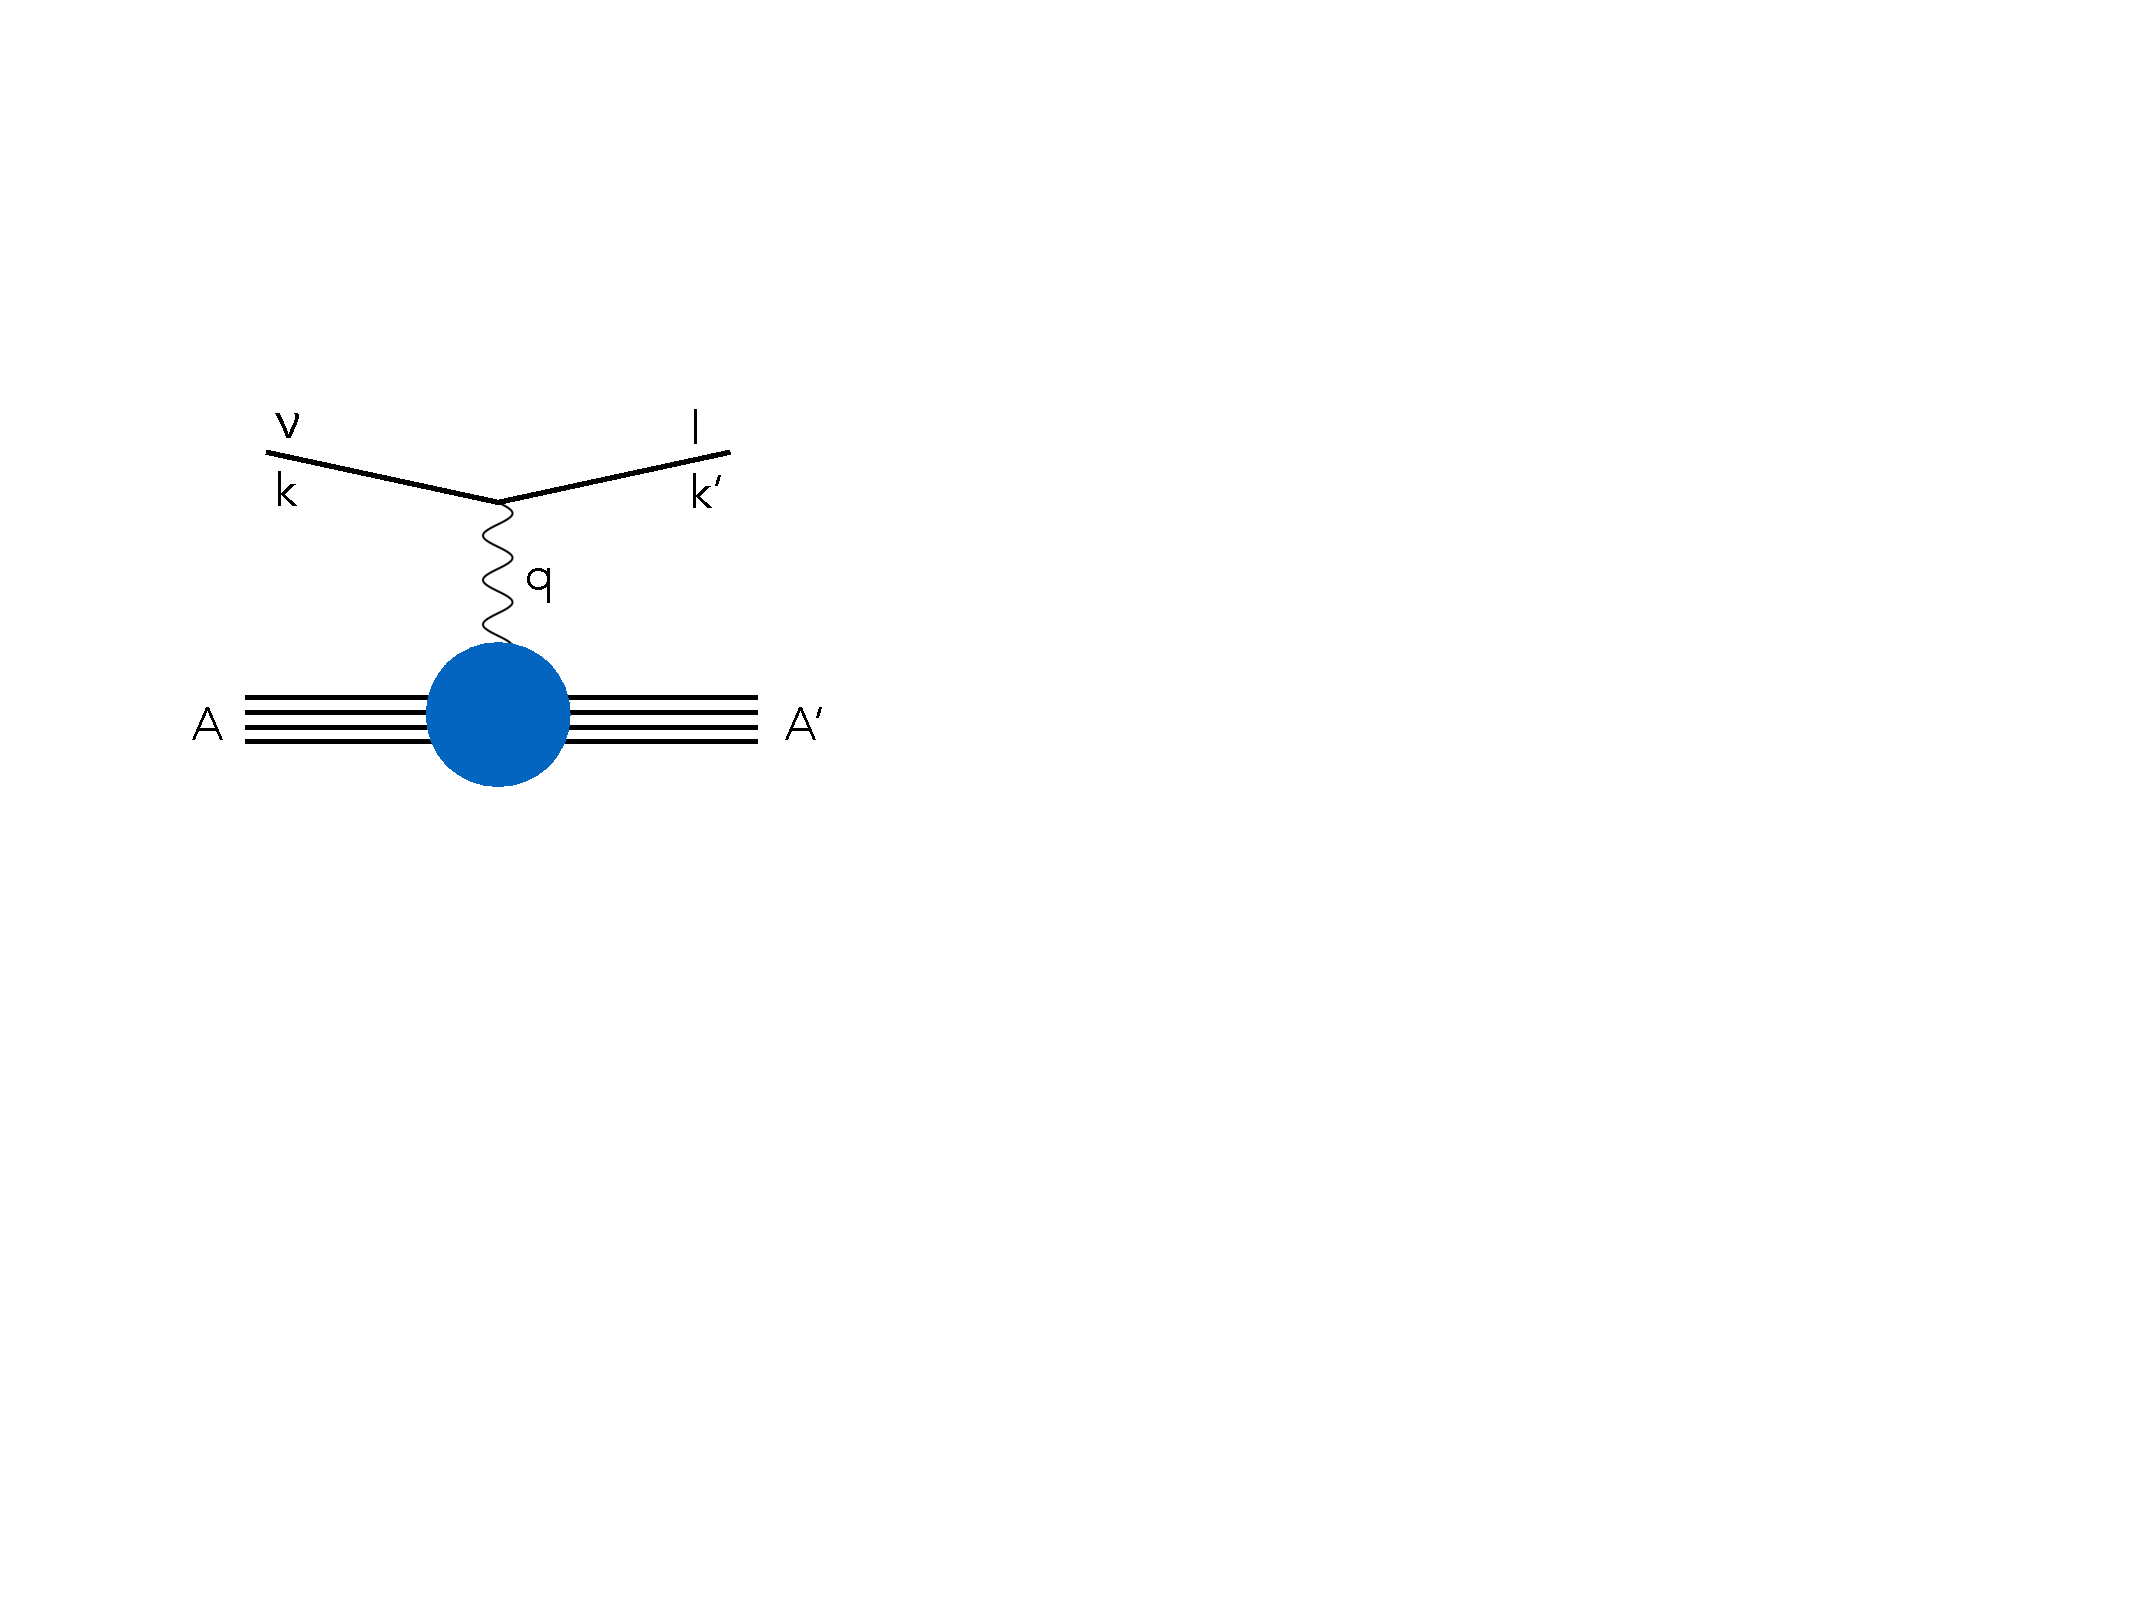
\includegraphics[height=.28\textwidth]{images/NeutrinoInteractions/impulse_approximation_a}
   \label{fig:impulse_approximation_a}} \quad\quad\quad
\subfloat[][]
   {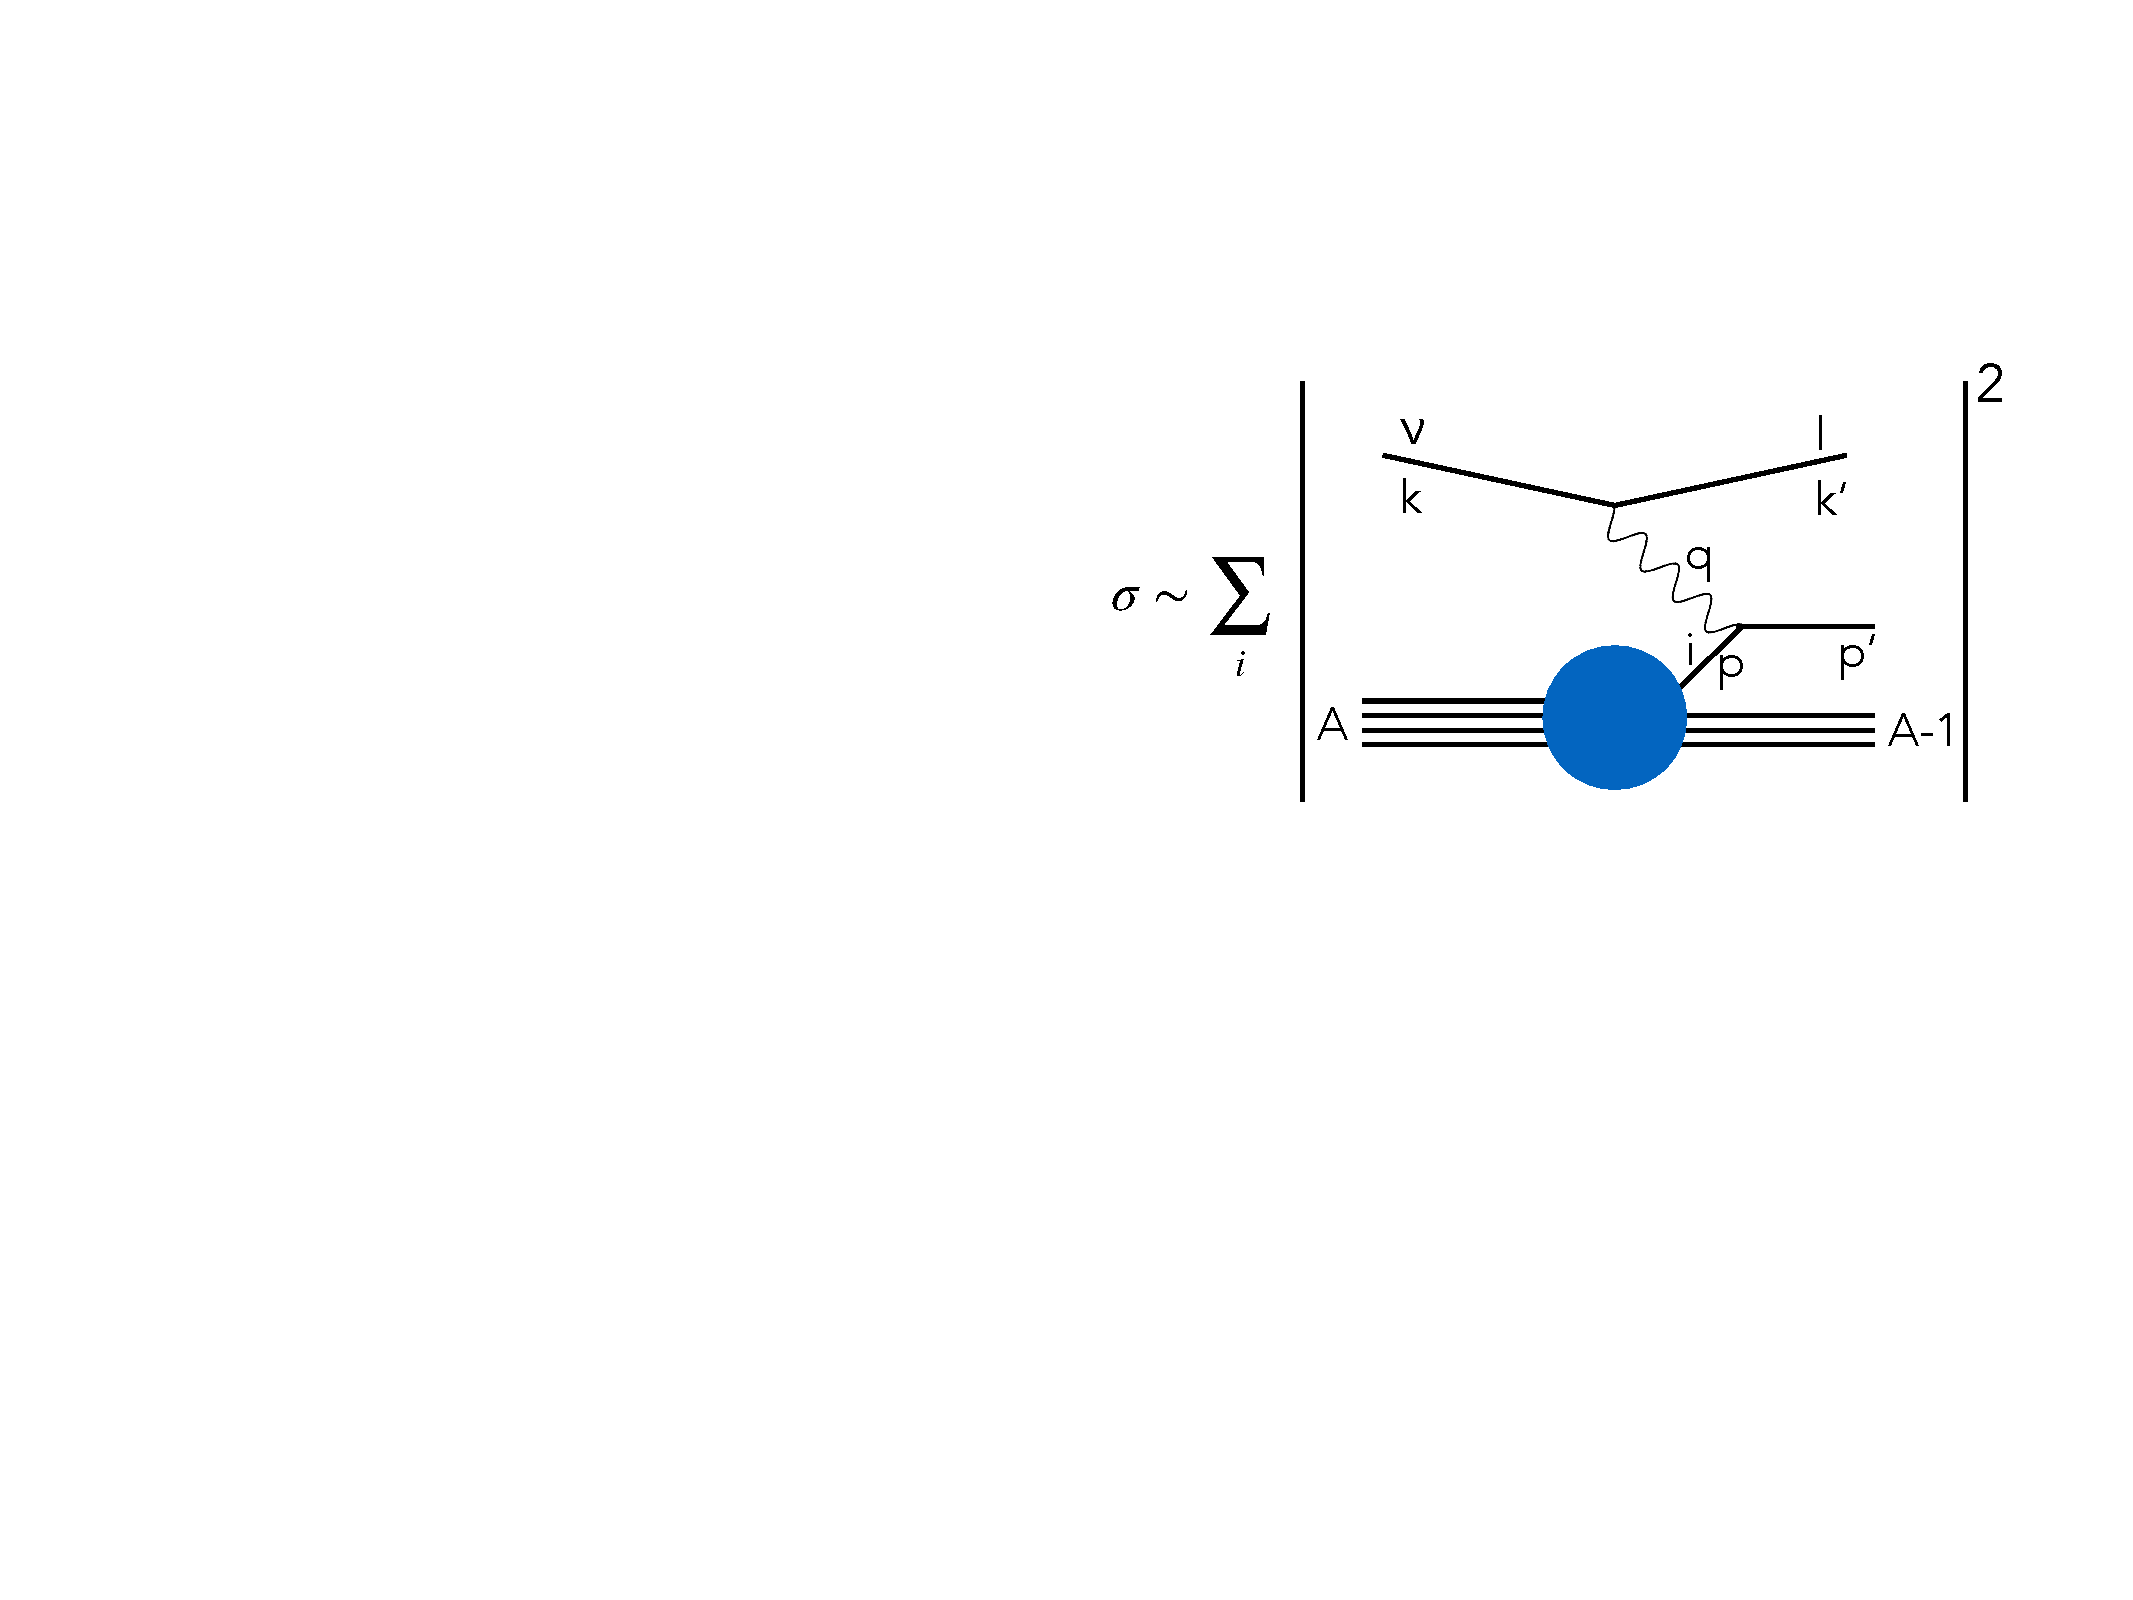
\includegraphics[height=.28\textwidth]{images/NeutrinoInteractions/impulse_approximation_b}
   \label{fig:impulse_approximation_b}} \\
\caption[Feynman Diagrams for the Impulse Approximation]{\protect\subref{fig:impulse_approximation_a}~Feynman diagram for the process $\nu_l + A \rightarrow l^- + A'$. \protect\subref{fig:impulse_approximation_b}~shows the \acrshort{ia} used to calculate the cross section for the process.}
\label{fig:impulse_approximation}
\end{figure}


In this approximation, the Fermi motion is embedded in the SF $P (\mathbf{p}, E)$, which needs to be characterised.
A simple and commonly used spectral function model is the global \acrfull{rfg} model~\cite{moniz}. Here, nucleons within the nucleus are modelled as non-interacting fermions inside a pervading nuclear potential, such that all momentum states are filled from the ground state upwards. The highest momentum state has momentum $p_F$, known as the Fermi momentum, which depends on the number of nucleons in a nucleus. 
This means that the \acrshort{sf} can be written as $P(\mathbf{p}, E) \propto \theta(p_F - |\mathbf{p}|)$, which then needs a Dirac $\delta$-function that ensures the conservation of energy. The energy of the struck nucleon (off-shell) can be written as:
\begin{equation}
E_\mathbf{p} = \sqrt{\mathbf{p}^2 + M^2} - \epsilon(\mathbf{p}),
\end{equation}
where $M$ is the nucleon mass and $\epsilon$ is the so-called interaction energy. The Smith–Moniz approach to the FG model \cite{moniz} is to approximate $\epsilon(\mathbf{p})$ by the constant average value $\bar{\epsilon}$, and conserve energy only on average. In this way, the spectral function takes the form
\begin{equation}
P(\mathbf{p}, E) = N \, \delta(\sqrt{\mathbf{p}^2 + M^2} - \bar{\epsilon} - M + E)\theta(p_F - |\mathbf{p}|),
\end{equation}
where $N$ is a normalisation constant. Overall, the Heaviside function gives rise to a sharp end in the \acrshort{sf} distribution, as can be seen from the green curve in Figure~\ref{fig:nucleon_momentum}, which shows the nucleon momentum distribution, defined as
\begin{equation}
\label{eq:np}
n(\mathbf{p}) = \int dE \, P(\mathbf{p}, E).
\end{equation}

\begin{figure}[]
\centering
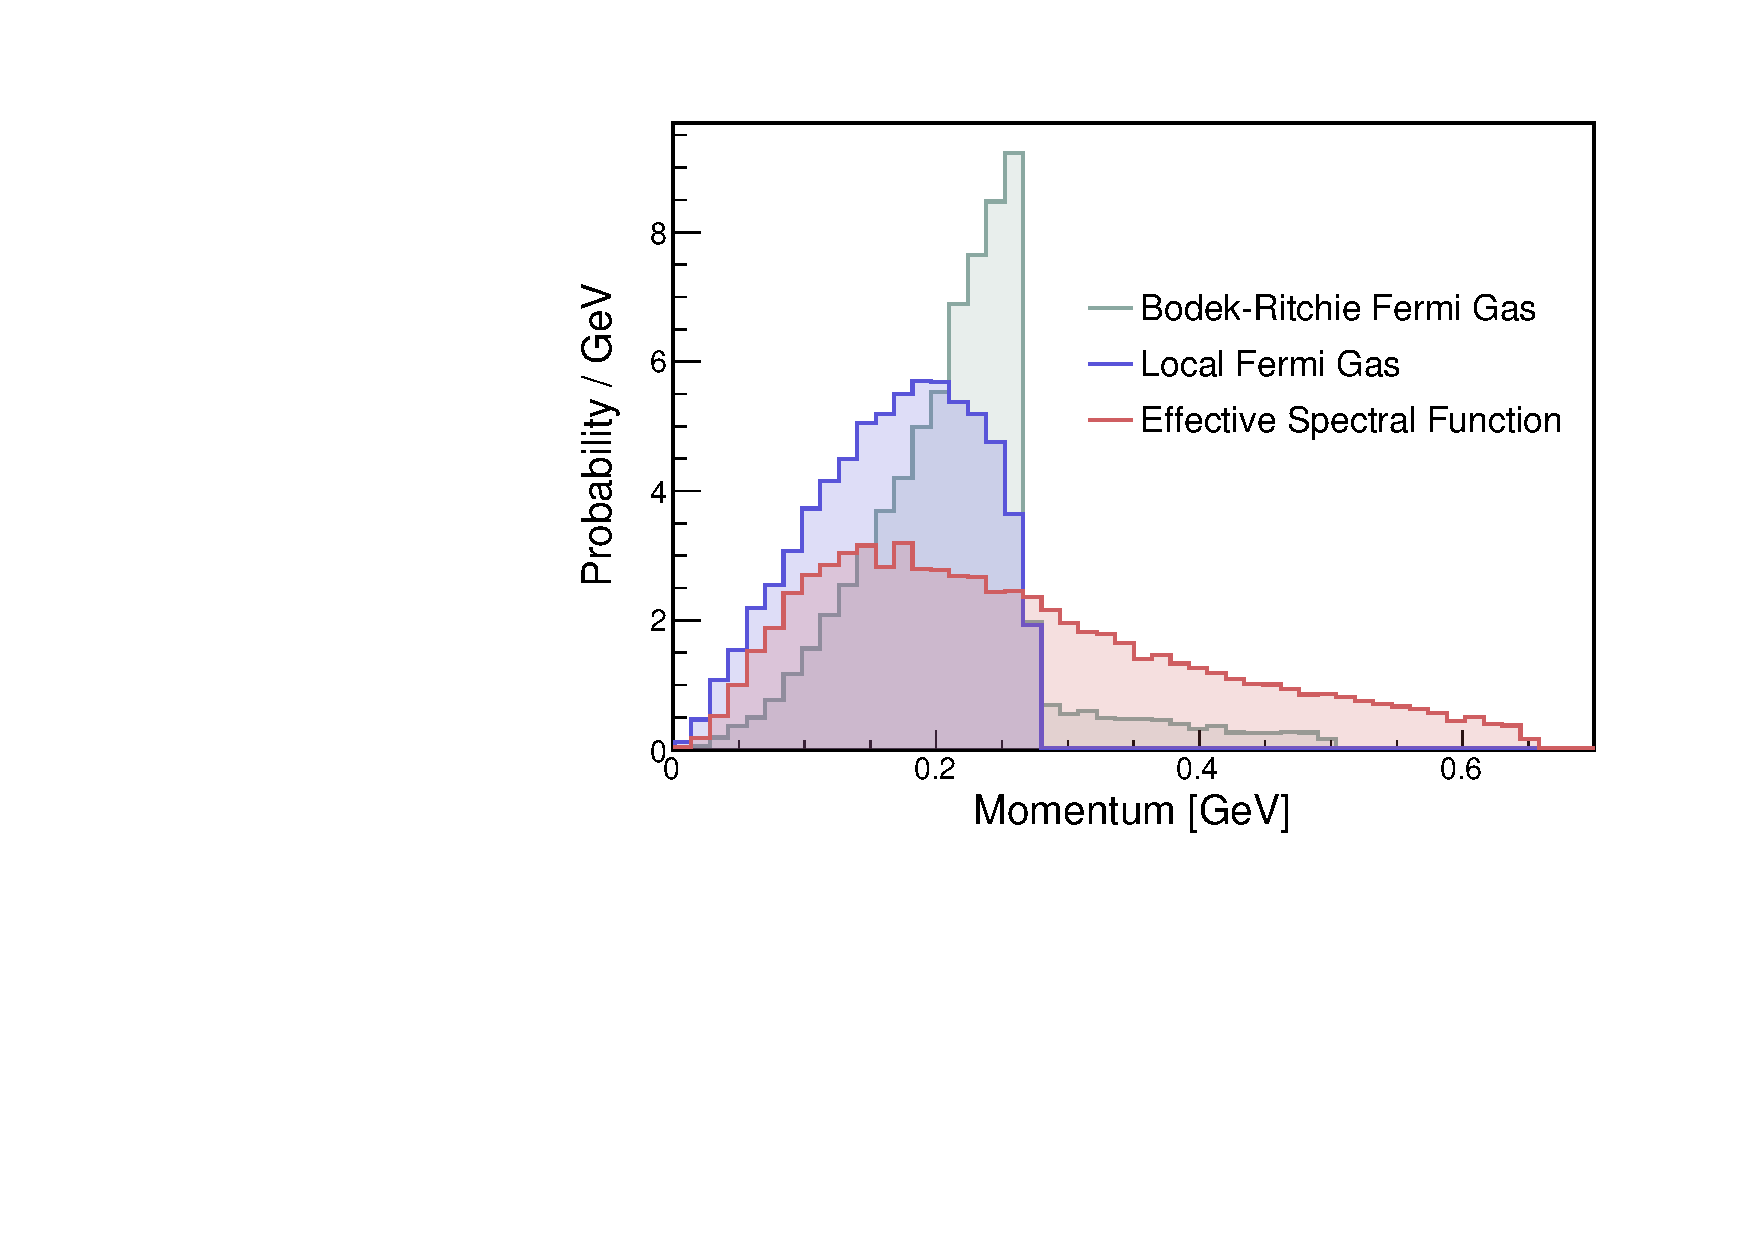
\includegraphics[width=.70\textwidth]{images/NeutrinoInteractions/nucleon_momentum}
\caption[Fermi Motion Distributions]{Nucleon momentum distributions in an argon nucleus for several spectral functions as implemented in the \g neutrino event generator. The Bodek-Ritchie Fermi gas, relativistic Fermi gas and effective spectral function are shown. The distribution shown is $4\pi |\bm{p}|^2n(|\bm{p}|)$ as a function of $|\bm{p}|$, with $n(\bm{p})$ given by Equation~\eqref{eq:np} and with normalisation condition given by $ 4\pi \int d|\bm{p}||\bm{p}|^2n(|\bm{p}|) = 1$.}
\label{fig:nucleon_momentum}
\end{figure}

The \acrshort{rfg} spectral function treats all nucleons as feeling the same constant binding potential, whilst in reality this depends upon the local density of the nucleus. More sophisticated \acrfull{lfg} spectral functions use the local nuclear density $\rho(r)$ to build a nuclear potential that depends on the radial position of a nucleon within the nucleus $r$, following the density profile of the nuclear matter~\cite{nieves_lfg}.

Although a \acrshort{lfg}  model is more realistic than an \acrshort{rfg}  model, nucleons are still treated as non-interacting fermions (other than via the local nuclear potential). However, it is well known from electron scattering data that nucleon-nucleon interactions inside the nuclear medium can significantly alter the distribution of the initial state nucleon momenta \cite{huberts, rohe}. Nucleon-nucleon correlations introduce a high-momentum tail in the \acrshort{sf}s. There are variations of the \acrshort{rfg} and \acrshort{lfg} that allow to include these correlations, one example is the Bodek-Ritchie modification to the \acrshort{rfg} model~\cite{bodek_ritchie_fermigas}. This is shown in Figure~\ref{fig:nucleon_momentum}, and is the main model used in this thesis.

Beyond the energy conserving Dirac-$\delta$ shown above, these models are not explicitly functions of the removal energy $E$. More sophisticated \acrshort{sf} can be extracted by taking into account two and three-nucleon interaction potentials which give rise to nucleon-nucleon correlations. These \acrshort{sf}, for examples the ones derived in~\cite{ia_approximation}, depend explicitly on $E$, and have a high momentum tail.

Effective SF have also been calculated \cite{esf} that are able to reproduce the predictions obtained by the superscaling variable \cite{superscaling}. This SF also has a high momentum tail, as shown in Figure~\ref{fig:nucleon_momentum}.

In general, Fermi gas models need an additional modification to take into account the effect of Pauli blocking. Since nucleons are fermions, they follow Fermi-Dirac statistics which allows only two nucleons per energy level. Scattering which would take the nucleon to a new state already occupied by other nucleons are not allowed. For \acrshort{qe} interactions, which change a neutron to a proton, enough energy has to be transferred to the proton to avoid this problem or the reaction does not take place. In the \g simulator~\cite{GENIE}, used in MicroBooNE and in the work presented in this thesis, a suppression factor is included based on the simple requirement that the momentum of the outgoing nucleon exceeds the Fermi momentum $k_F$ for the nucleus in question.

A summary of the nuclear models used in this thesis is shown in Section~\ref{sec:simulation}.



\subsection{Final State Interactions}

As described in the previous section, many generators employed by neutrino experiments adopt the \acrshort{ia} in which neutrinos scatter on individual quasi-free nucleons. In this picture any neutrino-nucleus interaction can be factorised in a two-step process: in the first step, the neutrino scatters on a bound nucleon, and in the second step \acrfull{fsi} affect the hadrons produced in the first step. \acrshort{fsi} happen as pions and protons rescatter before exiting the nucleus. As an example, Figure~\ref{fig:fsi} shows how pions can be absorbed, can be scattered elastically, can produce new pions, or can exchange electric charge with nucleons.

\begin{figure}[]
\centering
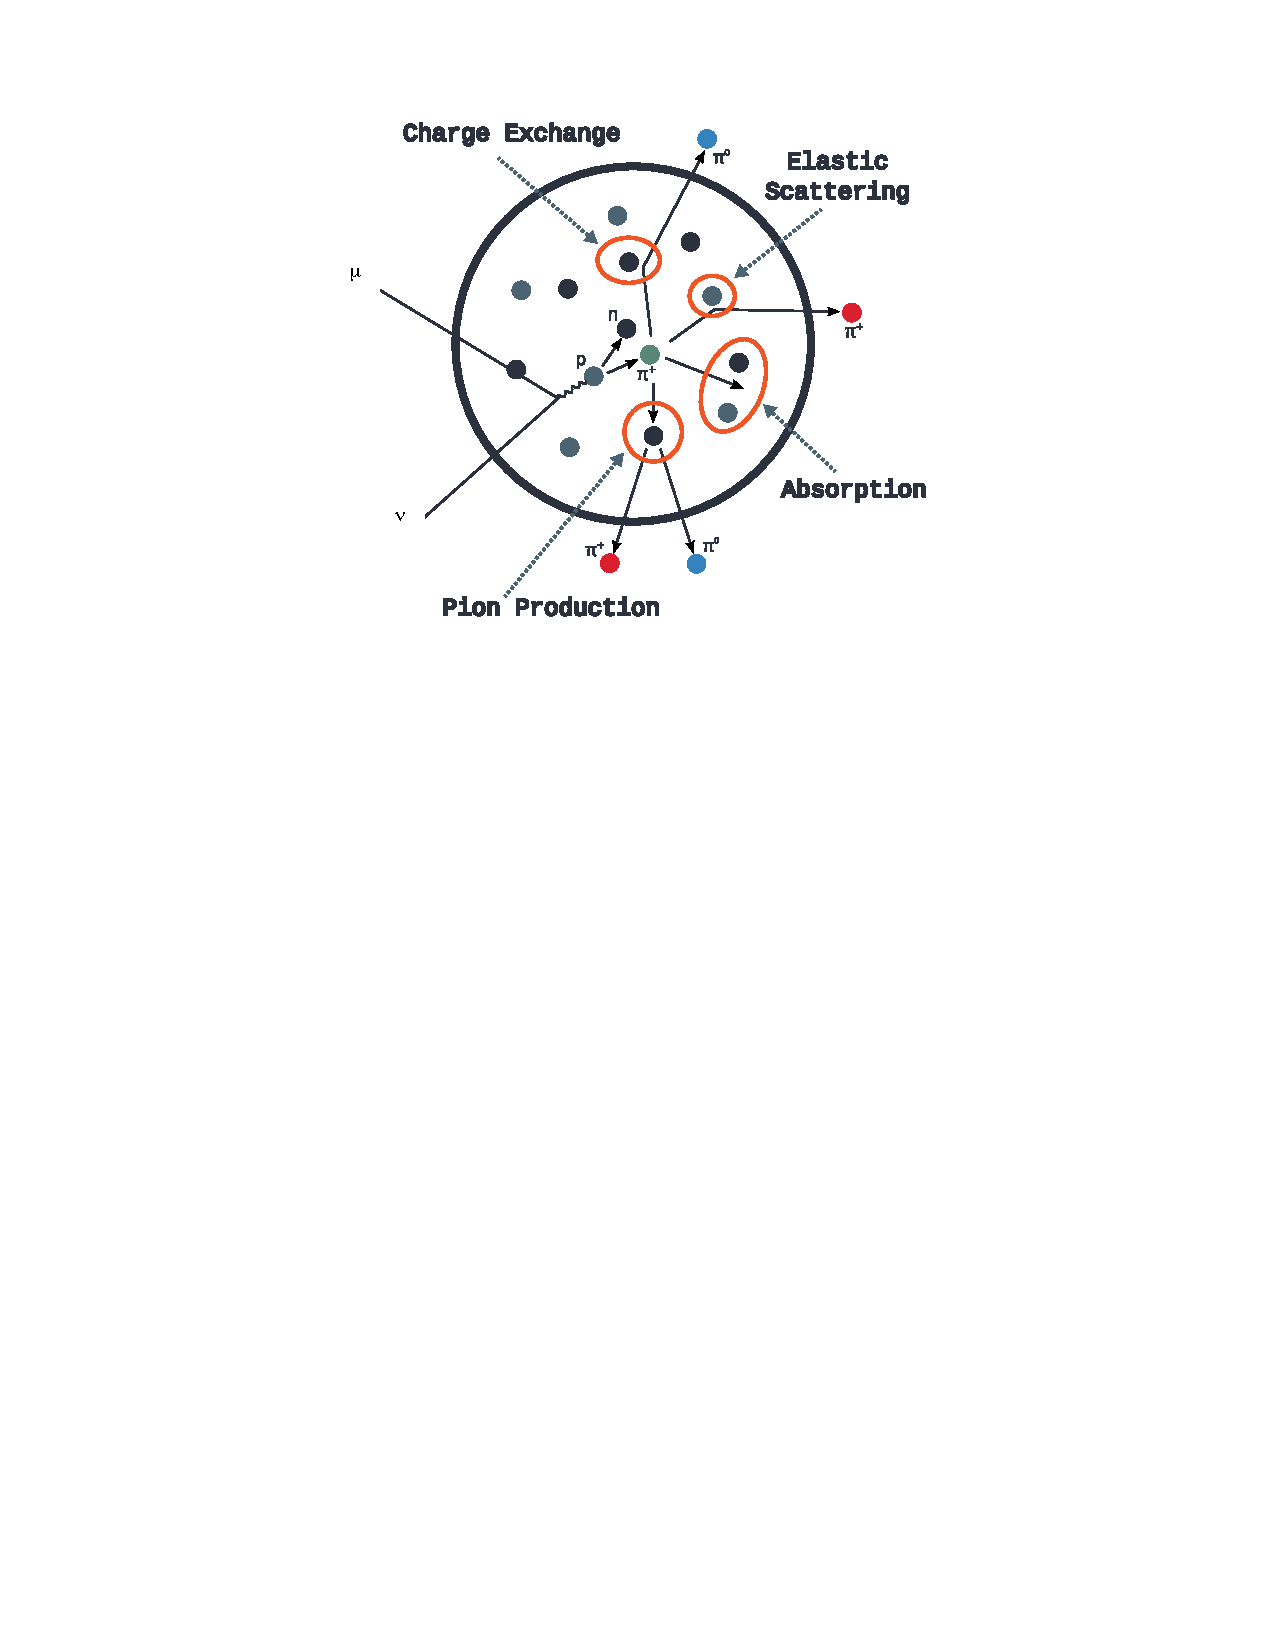
\includegraphics[width=.50\textwidth]{images/NeutrinoInteractions/fsi}
\caption[Cartoon of Final State Effects]{Hadrons produced at the neutrino interaction vertex must still traverse the dense nuclear matter and they are then subject to \acrshort{fsi} before appearing in the detector. The image shows how pions can be absorbed, scattered, produce new pions or exchange electric charge with other nucleons. A similar picture can be drawn for nucleons. Image credit: \cite{golan_thesis}.}
\label{fig:fsi}
\end{figure}

Simulations used in major neutrino oscillation experiments, in their description of \acrshort{fsi} effects, rely on the model of \acrfull{inc} \cite{inc}. These cascade models assume the nucleus is an ensemble of quasi-free nucleons and the incident particle interacts in a series of encounters with single nucleons called a cascade (see Figure~\ref{fig:fsi}).
All interactions are governed by the cross section for the free processes, and the probability of interaction is governed by a mean free path $\lambda = 1/(\sigma\cdot\rho(r))$. The probability for a multitude of different interactions (e.g. elastic scatter, charge exchange, absorption) is calculated at each step based on the local nuclear density and, if necessary, such an interaction is simulated. This continues until the hadron leaves the nucleus. These cascade models have some limitations, they use a simple Fermi gas model to describe the distribution of the nucleons, effects of nucleon correlations must be included empirically and both the struck nucleon and the scattered hadron are likely to be off-shell, while they are treated as free particles.

\acrshort{fsi}s contribute significantly to the systematic uncertainties in neutrino oscillation measurements as they are extremely difficult to model or constrain with experimental data. In the simulation used in this thesis (\g), the intranuclear transport is handled by a subpackage called INTRANUKE and the model used for the \acrshort{inc} is called \texttt{hA}~\cite{GENIE_reweighting}. Rather than calculate a cascade of hadronic interactions as is done in a complete \acrshort{inc} model, the \texttt{hA} model uses the total cross section for each possible nuclear process for pions and nucleons. This is an empirical and data-driven model \cite{GENIE_reweighting} which uses data from Fe targets and extrapolates to other targets.

To conclude this section, it is important to note the nucleus will also affect the lepton in the final state. For targets with atomic number $Z$ greater than one, the effect of the electric field of the nucleus on the scattered lepton must be considered. Corrections due to this electric field are called Coulomb corrections. The corrections result in an acceleration (for $l^+$) or deceleration (for $l^-$) of the scattered lepton $l$, thus resulting in a variation of its momentum.

In this work, the measured neutrino cross sections at MicroBooNE will be compared to two \g simulations: one which includes the \texttt{hA} cascade model and no Coulomb corrections, and another that includes an updated cascade model called  \texttt{hA2014}~\cite{genie_production_release} (which includes a wide range of data~\cite{ashery} for other nuclei than Fe for $\pi^{\pm}$ so that much less extrapolation is needed), and Coulomb corrections as calculated by Nieves et al.~\cite{nieves, nieves2}.



\subsection{Nucleon-Nucleon Correlations and the Random Phase Approximation}
\label{sec:rpa}

MiniBooNE neutrino cross-section measurements \cite{miniboone} were much larger than the theoretical predictions. This is shown in Figure~\ref{fig:numu_xsec}, where the MiniBooNE and the NOMAD measurements, both on carbon, appear to differ in normalisation by about 30\%. The low energy MiniBooNE results are higher than expected from the Fermi Gas model with more sophisticated impulse approximation calculations assuming an axial mass $M_A = 1.0$ GeV from deuterium-based measurements. Indeed, a large nucleon axial mass of $M_A = 1.35\pm0.17$ GeV was needed to describe these data. Such large values for $M_A$ were in clear conflict with other electron and neutrino experiments which result in a value very close to 1 GeV ($M_A = 1.014 \pm 0.014$ GeV \cite{ma_bodek}). This is shown in Figure~\ref{fig:miniboone_ma}, where data from MiniBooNE now show the measured differential cross section as a function of the muon kinetic energy, and the black line shows the prediction with an axial mass of 1.32 GeV. This is the so-called MiniBooNE $M_A$ puzzle. 

\begin{figure}[]
\centering
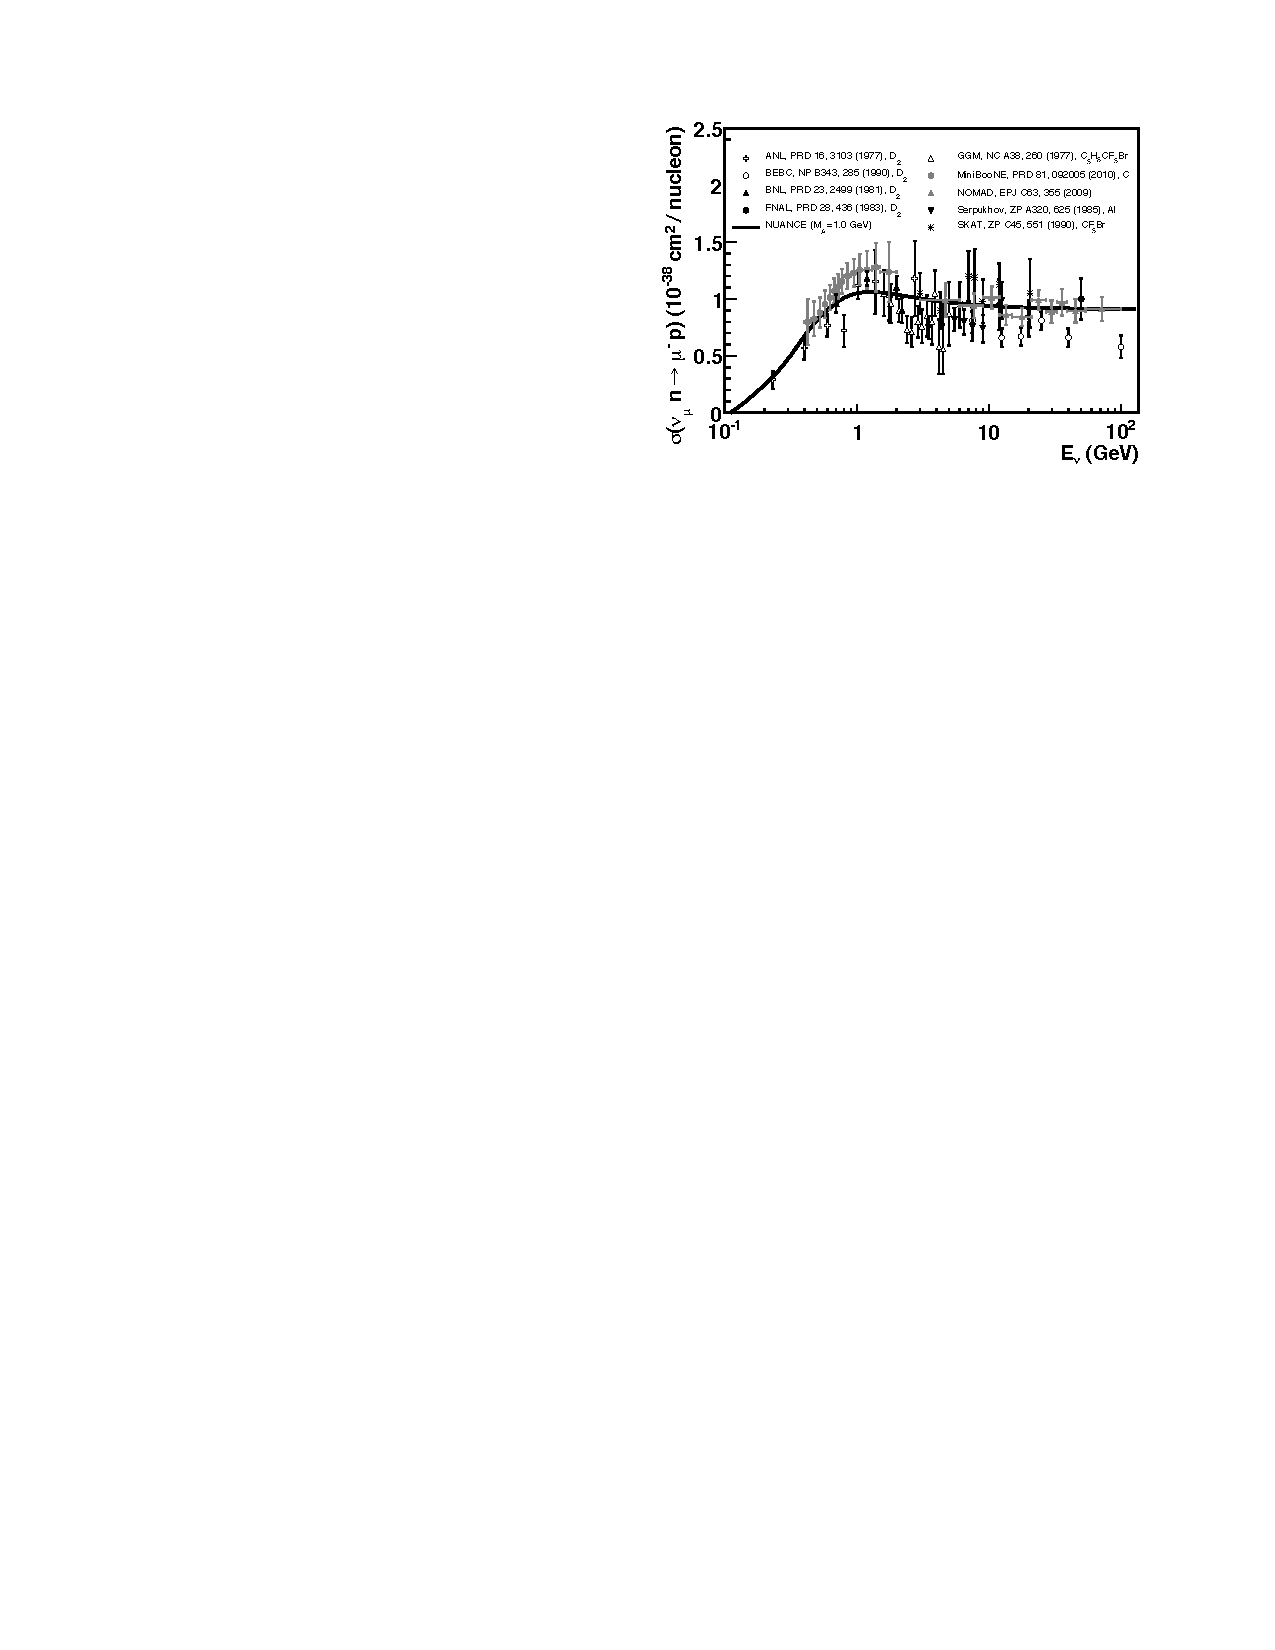
\includegraphics[width=.7\textwidth]{images/NeutrinoInteractions/numu_xsec}
\caption[Existing Measurements of the $\nu_\mu$ Quasi-Elastic-Like Scattering]{Existing measurements of the $\nu_\mu$ \acrshort{qe}-like scattering cross section, $\nu_\mu n\rightarrow\mu^-p$, as a function of neutrino energy on a variety of nuclear targets. The free nucleon scattering prediction assuming $M_A = 1.0$ GeV is shown for comparison. Figure from \cite{zeller}.}
\label{fig:numu_xsec}
\end{figure}

It is currently believed that nuclear effects beyond the impulse approximation approach are responsible for the discrepancies noted in the experimental data. A more theoretically sound solution to the puzzle was obtained thanks to the inclusion of some standard nuclear effects such as multinucleon mechanisms~\cite{nieves_ma}.
In these mechanisms, the $W$ boson can be absorbed by nucleons belonging to correlated pairs and to two-nucleon currents arising from \acrfull{mec} which lead to the excitation of multinucleon or $2p2h$ (2-particles 2-holes) excitations. In these models, a substantial part of the cross section measured corresponds to events in which at least two nucleons are emitted.
The consideration of the $2p2h$ nuclear excitations allows to describe the MiniBooNE cross section $d\sigma/dT_\mu/d\cos\theta_\mu$ with values of $M_A$ around 1 GeV, as can been seen from the green curve in Figure~\ref{fig:miniboone_ma}.

\begin{figure}[]
\centering
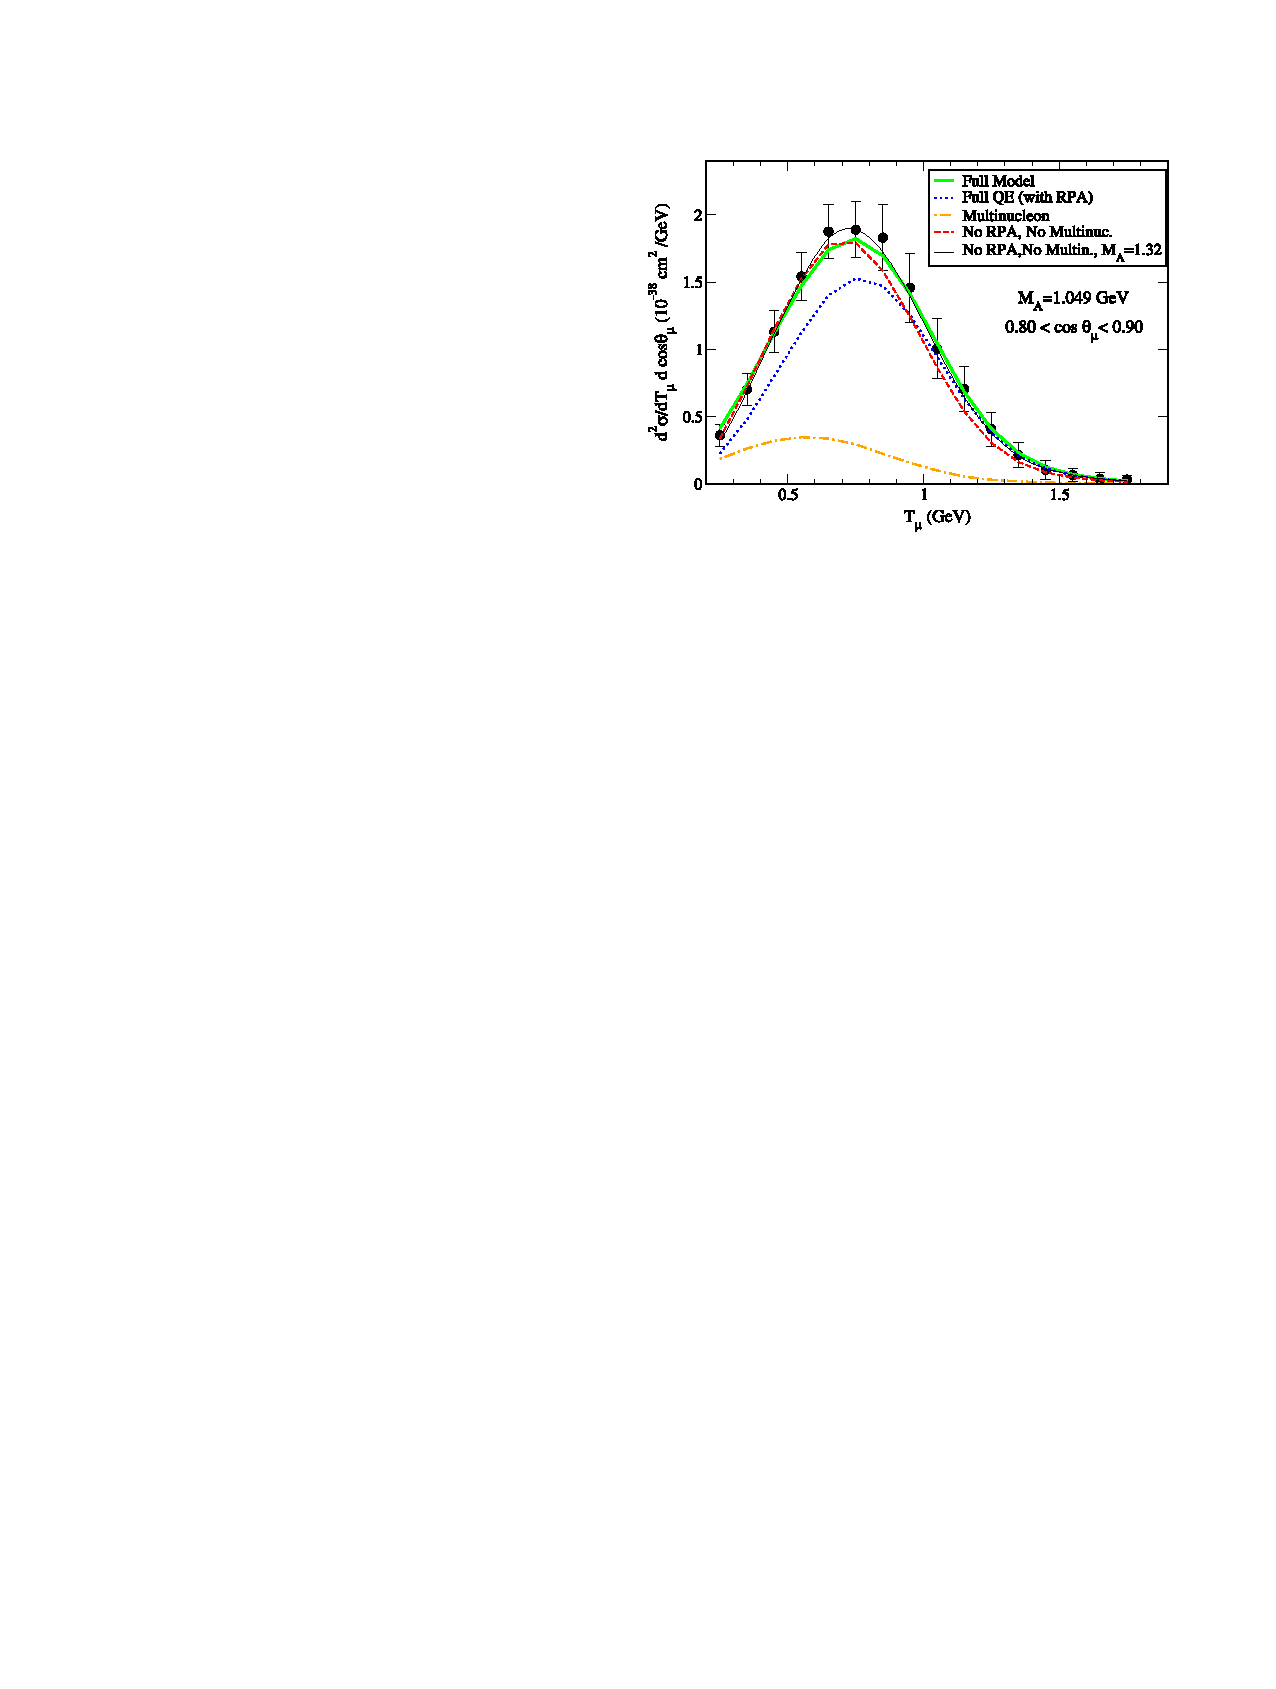
\includegraphics[width=.7\textwidth]{images/NeutrinoInteractions/miniboone_ma}
\caption[MiniBooNE Cross Section and Predictions]{The muon angle and energy distribution $d^2\sigma/d\cos\theta_\mu dT_\mu$ for $0.80 < \cos\theta_\mu < 0.90$ from the MiniBooNE experiment \cite{miniboone}. The curves show different model predictions: the black line show the \acrshort{mc} obtained by increasing $M_A$ to 1.35 GeV, while the green line shows the model prediction with multinucleon effects and \acrshort{rpa} included. The two predictions are similar. Figure from \cite{nieves_ma}.}
\label{fig:miniboone_ma}
\end{figure}

However, not only multinucleon mechanisms but also \acrfull{rpa} corrections~\cite{nieves} turn out to be essential to find that axial masses consistent with the world average lead to a good description of the MiniBooNE data. 
\acrshort{rpa} is a method to describe microscopic quantum mechanical interactions in complex many-body systems. In this case, the many-body system is described by the mutual interactions of nucleons inside the nucleus, which cannot be resolved exactly. The overall effect of \acrshort{rpa} correlations is to account for the change of the electroweak coupling strengths, from their free nucleon values, due to the presence of strongly interacting nucleons.
\acrshort{rpa} corrections are dominant at low $Q^2$: the $W$ or $Z$ probe has small resolution and sees nucleons embedded in the nuclear potential. While at higher $Q^2$ \acrshort{rpa} corrections are negligible as the probe has high resolution and sees nucleons as almost free particles.

The cross section measurements presented in this thesis are compared to a default \g simulation that does not include \acrshort{rpa} and that uses an empirical model for the simulation of \acrshort{mec} events that reproduces MiniBooNE and NOMAD data~\cite{mec_dytman}. Moreover, the measurements are also compared  to an alternative configuration of \g that uses the Nieves et al. model~\cite{nieves, nieves2}, which folds interactions of correlated pairs and a \acrshort{rpa} corrections to describe interactions of many bodies into the calculation.





%\begin{SCfigure}[]
%\centering
%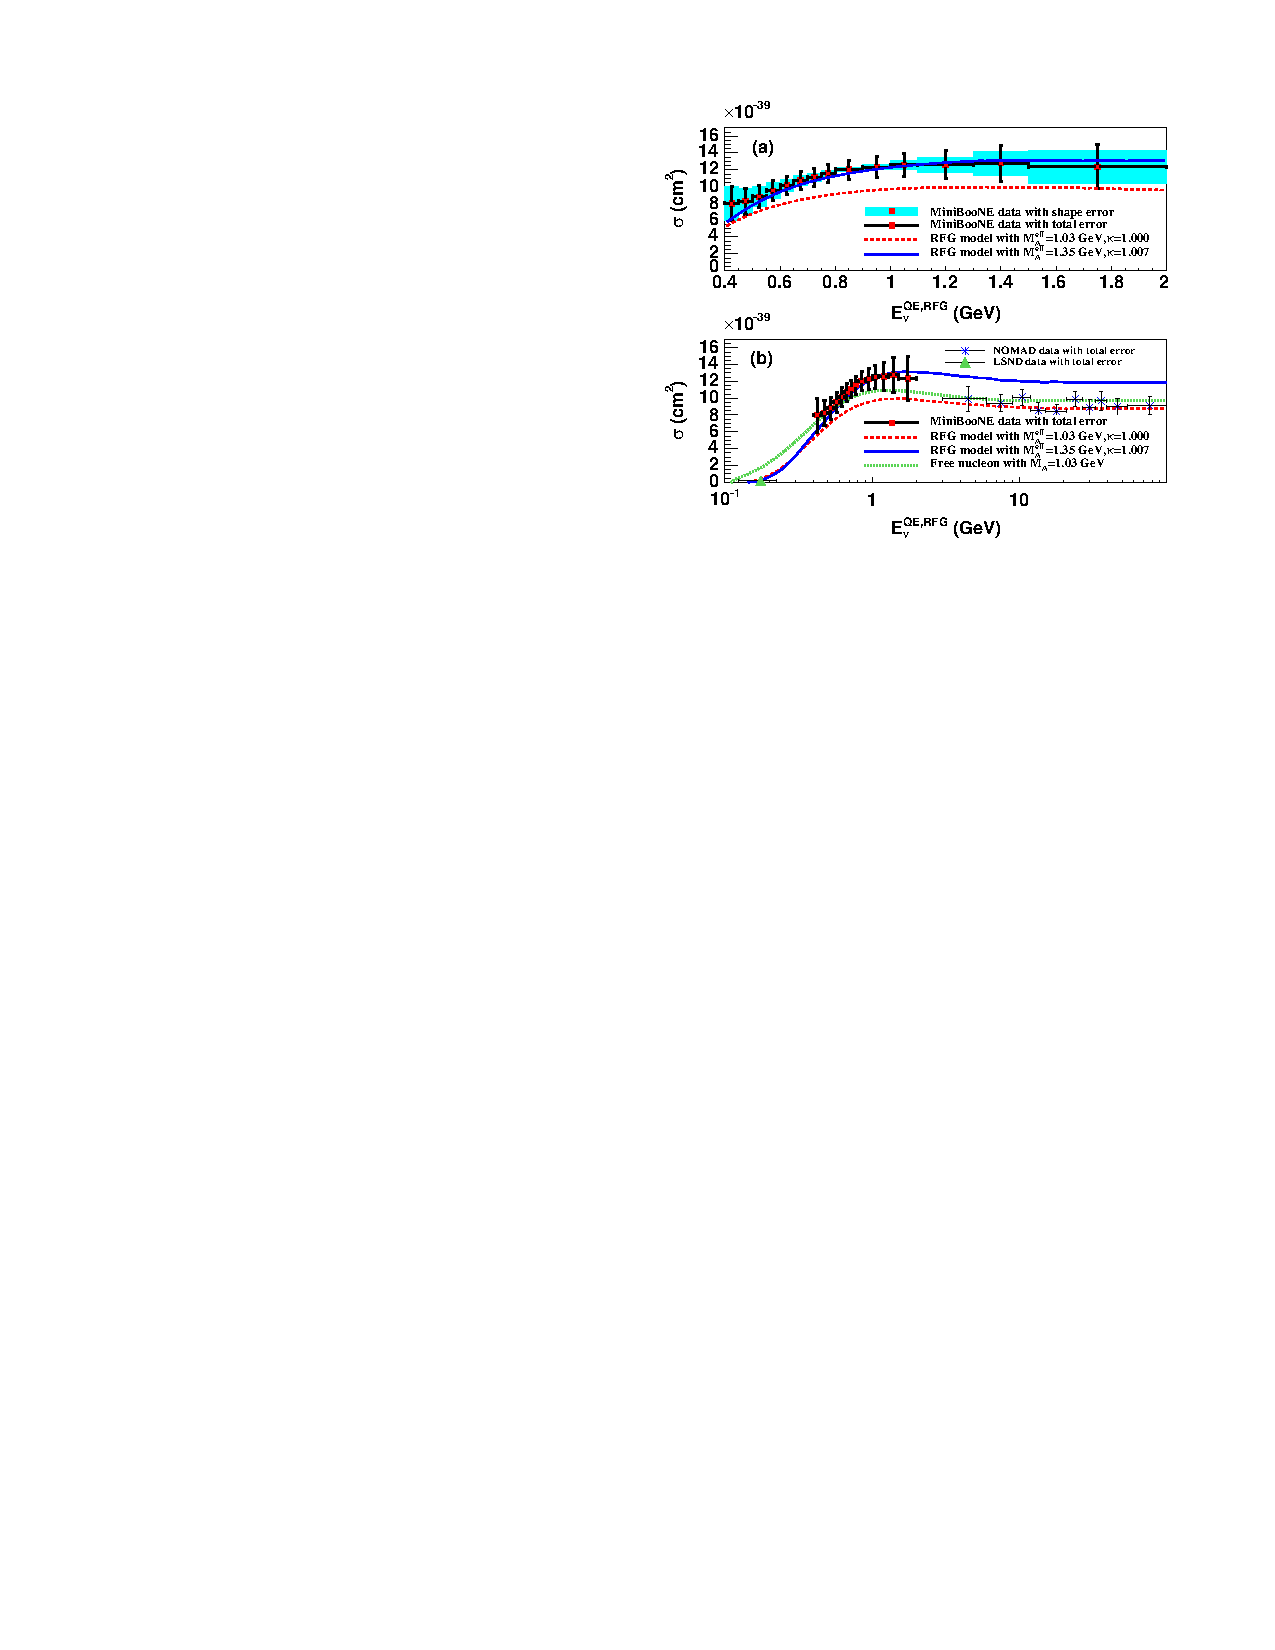
\includegraphics[width=.58\textwidth]{images/NeutrinoInteractions/miniboone}
%\caption{MiniBooNE cross section as a function of neutrino energy. In (a), shape errors are shown as shaded boxes along with the total errors as bars. In (b), a larger energy range is shown along with results from the LSND [56] and NOMAD [10] experiments. Also shown are predictions from the NUANCE simulation for an RFG model with two different parameter variations and for scattering from free nucleons with the world-average MA value.  Figure from \cite{miniboone}.}
%\label{fig:miniboone}
%\end{SCfigure}



%\begin{SCfigure}[]
%\centering
%\includegraphics[width=.50\textwidth]{images/NeutrinoInteractions/rpa}
%\caption{the \acrshort{rpa} correction factor as a function of $Q^2$}
%\label{fig:rpa}
%\end{SCfigure}





\section{Final Remarks}
\label{sec:remarks}

While most of our knowledge of neutrino cross sections around the $\sim 1$ GeV energy range comes from early experiments that collected relatively small data samples~\cite{zeller}, current experiments use heavy nuclei as target material, like hydrocarbon in the T2K and NO$\nu$A detectors, and argon in MicroBooNE. As described in the previous sections, nuclear effects seriously complicate the understanding of neutrino interactions and can greatly affect the sensitivity of neutrino oscillation experiments. 

Although many of the future experiments, such as DUNE~\cite{dune1, dune2, dune3} and the SBN program~\cite{sbn}, will all employ the \acrfull{lartpc} detection technology with argon as target material, experimental data for the neutrino-argon scattering process is scarce~\cite{ArgoNeuTCCincl, ArgoNeuTCCincl2}.

This thesis presents the first $\nu_{\mu}$ \acrshort{cc} inclusive measurement on argon at $\sim 0.8$~GeV of mean neutrino energy. The \acrshort{cc} inclusive channel is sensitive to some of the nuclear effects described in the previous sections and will be extremely valuable to future neutrino oscillation experiments. The signal topology for a $\nu_{\mu}$ \acrshort{cc} inclusive measurement is the presence and identification of a neutrino-induced muon track with or without accompanying particles. It is, therefore, the most inclusive cross section measurement that one can make, and due to the very clear signal definition allows straight-forward comparisons to theoretical models and other experiments. 

It is important to evaluate neutrino cross sections as a function of the kinematics of the outgoing muon as nuclear models will shape these distributions. Neutrino experiments have measured single differential cross sections as a function of the muon momentum ($d\sigma/dp_\mu$) or the cosine of the muon angle w.r.t.~the neutrino direction ($d\sigma/d\cos\theta_\mu$). Recently, experiments are also producing double-differential cross sections ($d^2\sigma/dp_\mu d\cos\theta_\mu$) as they provide a better insight in the properties of neutrino interaction with the nucleus and how the angle and the momentum of the lepton are correlated. For this reason, the analysis in this thesis will show both single and double-differential cross sections.

Some other modern experiments 
have also measured the $\nu_\mu$ \acrshort{cc} inclusive cross section. ArgoNeuT \cite{ArgoNeuTCCincl, ArgoNeuTCCincl2} and the T2K on-axis detector INGRID \cite{T2KCCinclINGRID,T2KCCinclINGRID2} published flux-integrated measurements. ArgoNeuT is the only experiment that published cross sections for neutrino-argon scattering to date, but at higher neutrino energy, around 5 GeV. SciBooNE \cite{SciBooNECCincl}, NOMAD \cite{NOMADCCincl}, MINOS \cite{MINOSCCincl}, and MINERvA \cite{MINERvACCincl,MINERvACCincl2} all published \acrshort{cc} inclusive cross sections as a function of a reconstructed neutrino energy. The only experiments with published double-differential data are event distributions from SciBooNE \cite{SciBooNECCincl} and cross section measurements from the T2K on-axis detector \cite{T2KCCinclND280}, both as a function of muon angle and muon momentum. T2K -- which has comparable beam energy to MicroBooNE -- was able to bin in four angular and five momentum bins. All flux-integrated or energy-dependent measurements are summarised in Figure~\ref{fig:pdg_cross_sections} from the PDG review article \cite{PDGReview}. This analysis provides a flux integrated measurement that can be added to a future Figure~\ref{fig:pdg_cross_sections}, as well as single differential and double differential cross sections as a function of muon momentum and angle, which allow to test generator predictions.

%\begin{SCfigure}[]
%\centering
%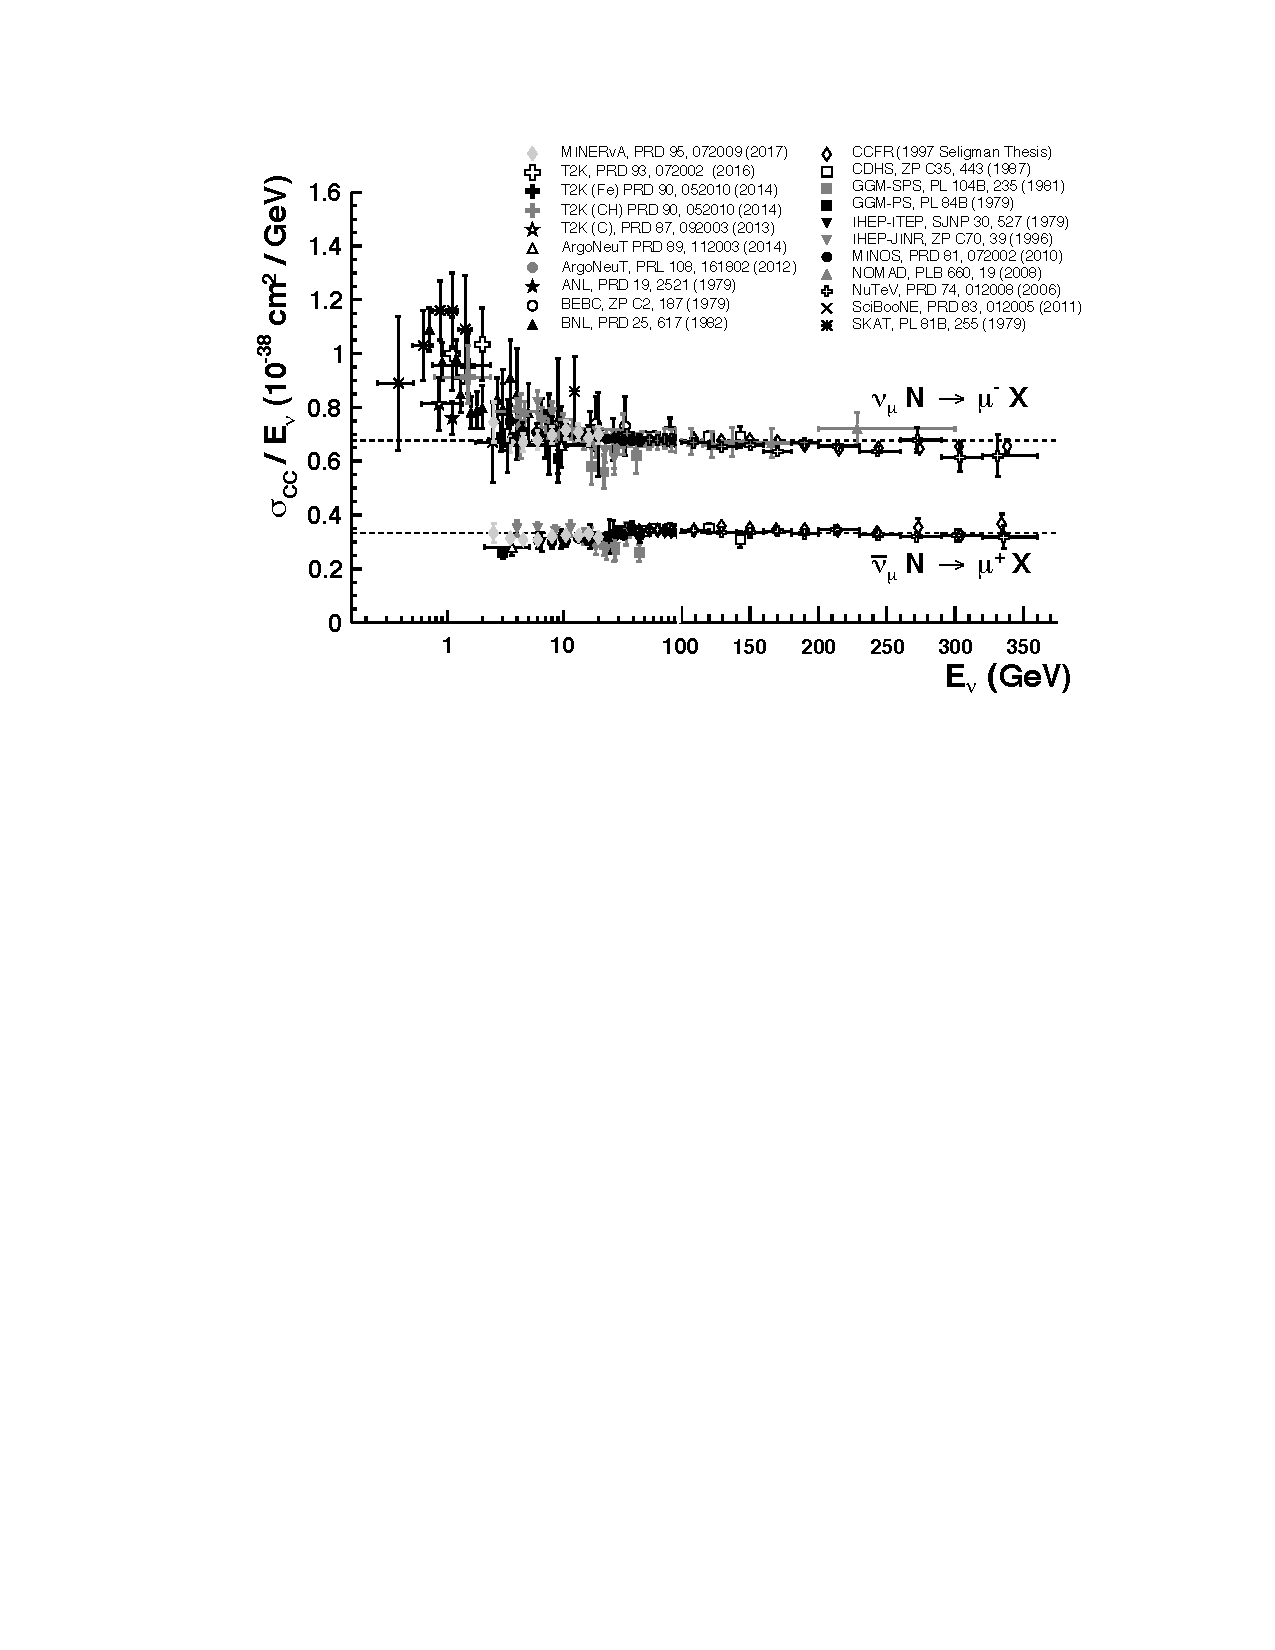
\includegraphics[width=.50\textwidth]{images/NeutrinoInteractions/pdg_cross_sections}
%\caption{Measurements of per nucleon $\nu_\mu$ and $\bar{\nu}_\mu$ \acrshort{cc} inclusive scattering cross sections divided by neutrino energy as a function of neutrino energy. From \cite{PDGReview}.}
%\label{fig:pdg_cross_sections}
%\end{SCfigure}

\begin{figure}[t]
\centering
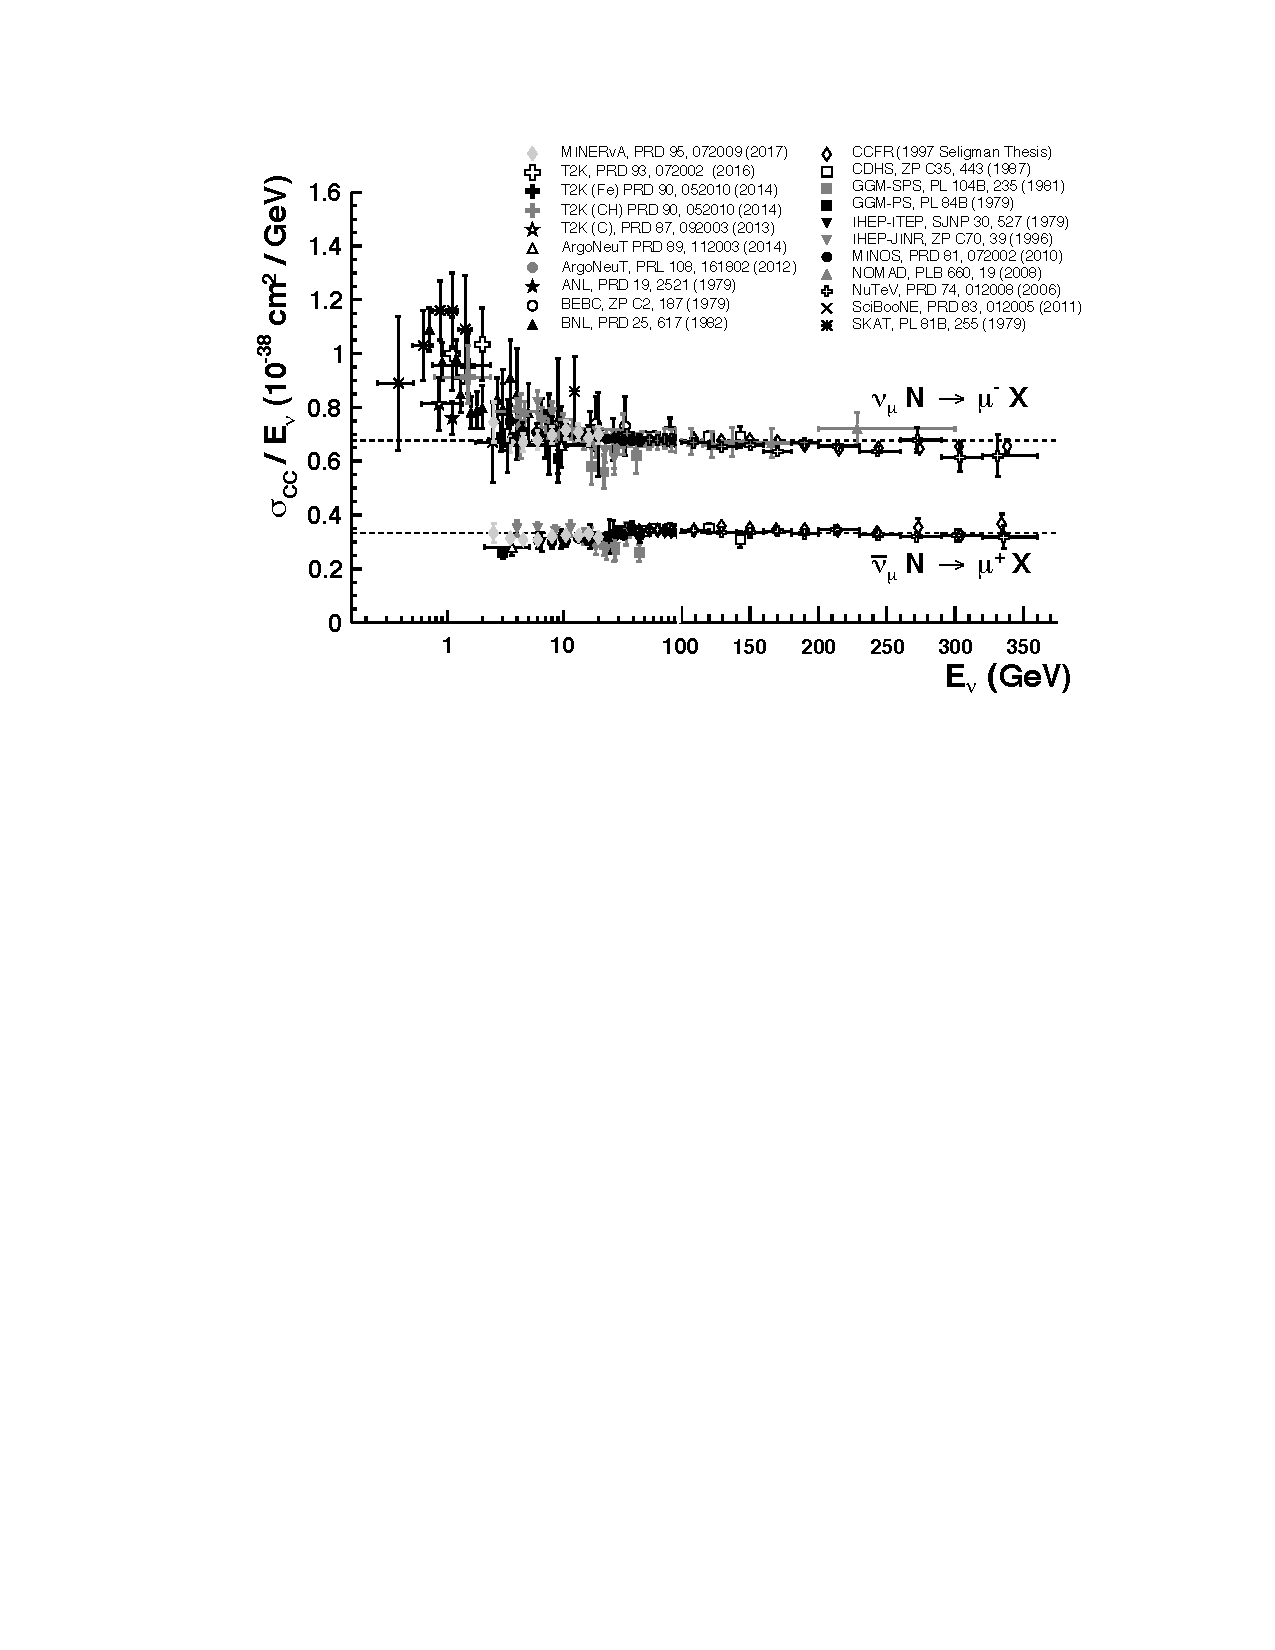
\includegraphics[width=1.0\textwidth]{images/NeutrinoInteractions/pdg_cross_sections}
\caption[Measurements of $\nu_\mu$ and $\bar{\nu}_\mu$ Charged Current Inclusive Scattering]{Measurements of per nucleon $\nu_\mu$ and $\bar{\nu}_\mu$ \acrshort{cc} inclusive scattering cross sections divided by neutrino energy as a function of neutrino energy. From \cite{PDGReview}.}
\label{fig:pdg_cross_sections}
\end{figure}

















